\documentclass[useAMS,usenatbib]{mn2e}
\usepackage[]{natbib,amsmath,amssymb,times,refname}
\bibpunct{(}{)}{;}{a}{}{,}
%\linespread{1.0}
%\usepackage[utf8]{inputenc}
\usepackage{tabularx,amsmath,amssymb,hyperref}
\usepackage{graphicx,epsfig,color,latexsym}


\renewcommand{\d}{\mathrm{d}}
\newcommand{\e}{\mathrm{e}}
\newcommand{\ii}{\mathrm{i}}
\newcommand{\bea}{\begin{eqnarray}}
\newcommand{\eea}{\end{eqnarray}}
\newcommand{\be}{\begin{equation}}
\newcommand{\ee}{\end{equation}}
\newcommand{\rund}[1]{\left(#1\right)}
\newcommand{\vc}[1]{\mbox{\boldmath $#1$}}
\newcommand{\dc}{\partial}
\newcommand{\eck}[1]{\left[ #1 \right]}

\newcommand{\msun}{\,h^{-1}\,M_{\odot}}
\newcommand{\iobs}{I^{\rm obs}}

\long\def\/*#1*/ {}

%\def\llabel#1{\label{sc:#1}  {#1}\hspace{0.5cm}}
%\def\elabel#1{\label{eq:#1}\fbox{#1}}
\def\llabel#1{\label{sc:#1}}
\def\elabel#1{\label{eq:#1}}

\sloppy

\title[Colour gradient bias]
{Calibration of colour gradient bias in shear measurement using CANDELS}
\author[Xer et al.]%
{
X. Er$^1$ \thanks{er.xinzhong@oa-roma.inaf.it},
H. Hoekstra$^2$, T. Schrabback$^3$, V. F. Cardone$^1$, R. Scaramella$^1$, R. Maoli$^4$,
\newauthor{M. Vicinanza$^{1,4,5}$, B. Gillis$^{6}$ L. Miller$^{7}$, J. Rhodes$^{8,9}$}
\\
$^1$ I.N.A.F. - Osservatorio Astronomico di Roma, via Frascati 33, 00040 - Monte Porzio Catone, Roma, Italy\\
$^2$Leiden Observatory, Leiden University, PO Box 9513, NL-230 RA, Leiden, the Netherlands \\
$^3$Argelander Instutite fuer Astronomie, Auf dem Huegel 71, D-53121 Bonn, Germany\\
$^4$Dipartimento di Fisica, Universita di Roma "La Sapienza", Piazzale Aldo Moro, 00185 - Roma, Italy\\
$^5$Dipartimento di Fisica, Universita di Roma "Tor Vergata", via della Ricerca Scientifica 1, 00133 - Roma, Italy\\
$^6$Royal Observatory, University of Edinburgh, Blackford Hill, Edinburgh EH9 3HJ, UK\\
$^7$Department of Physics, Oxford University, keble Road, Oxford OX I 3RH, UK\\
$^8$Jet Propulsor Laboratory, California institute of Technology, 4800 Oak Grove Drive, Pasadena, CA 91109, USA\\
$^8$California Institute of Technology, 1200 East California Blvd, Pasadena, CA 91125, USA
%$$
}
\date{Accepted --;  received --;  in original from \today}
\pubyear{2016}

\begin{document}
\maketitle

\begin{abstract}
  In weak gravitational lensing, the precision strongly depends on
  the shape measurement of the galaxy images. Observation using wide
  band filter can provide images with high signal-to-noise ratio, and
  can cover a large redshift range as well. However, the shape
  measurement requires analysis of the point spread function
  (PSF). In general, both the PSF and the galaxy are chromatic,
  i.e. the shapes vary with wavelength. Thus, measuring the shape of
  galaxies using integrated images over the filter will cause higher
  order systematic bias, which is called colour gradient bias.
  %
  We perform an estimate of this bias using both simulated
  images and real data from CANDELS. We show that the estimation for
  colour gradient bias using two narrow bands can reach a high precision
  in the simulated noisy data. The estimation using noisy images has a
  large scatter, which may over-estimate the magnitude of the bias.
  In our sample of real galaxy images, we find correlations between
  the bias with the colour and the size of the galaxy. Moreover, we
  find that the higher order image distortions, such as flexion, will
  enlarge the colour gradient bias in shear, although it affects
  the estimation only when the images are in strong lensing regions.
\end{abstract}
\begin{keywords} cosmology, weak lensing, systematics
\end{keywords}

%\vspace{1.0\baselineskip}

\section{Introduction}

Weak gravitational lensing has been identified as a powerful method in
cosmology, such as mapping the large scale structures. The images of
distant galaxy are distorted by the gravitational potential generated
by the intervening matter. A statistical analysis of image distortion
of background galaxies provides crucial information about the mass
distribution and thus tight constraint to the cosmological models
\citep[e.g.][]{2001PhR...340..291B,2008ARNPS..58...99H}.

The precision of measuring the shapes of the galaxy images is limited
due to the atmospheric turbulence, i.e. Point Spread Function
(PSF). Thus space telescopes can take the advantage of small space
PSF, e.g. the future weak lensing survey loaded on the Euclid
satellite. The weak lensing survey by Euclid plans to provide a large
sample of accurate measurements of both shape and photometric redshift
for the galaxies. The filter of the Euclid image survey has a very wide
bandpass ($550nm-920nm$), which covers a large range of redshift of
galaxies and can also obtain galaxy images with high signal-to-noise
ratio (SNR).

In shear measurements, the galaxy shape is corrected using the
effective (integrated) PSF. However, the galaxies in general have
different intrinsic shapes at different wavelengths, as well as the
PSF, e.g. the size of PSF is slightly larger at longer wavelength.
\citep{2015ApJ...807..182M} have also shown that the differential
chromatic refraction can introduce systematics to the measurement of
galaxy shapes.  The chromatic PSF causes a bias in the measurement,
which can be estimated and reduced to the required levels using a
colour weighted PSF \citep{2010MNRAS.405..494C}. While the correction
described in \citet{2010MNRAS.405..494C} assumes a uniform spectral
energy distribution (SED) of the source galaxy. It becomes inaccurate
when the SED, or colour of the source galaxy varies spatially.  The
effects introduce a higher order systematic bias in measuring the
shape of galaxies, if one uses the integrated images and integrated
PSF. The bias, which we called colour gradient (hereafter CG) bias,
has dependence on several factors: such as the SED of the galaxy, the
relative size of the galaxy to the PSF, as well as the bandwidth of
the filter. The relative magnitude of the CG can be neglected for
narrow band survey. However, the CG bias is expected to be relevant
for Euclid, especially since the error budget of Euclid weak lensing project
is small \citep[e.g.][]{2013MNRAS.431.3103C,2013MNRAS.429..661M}.

In \citep{2012MNRAS.421.1385V, 2013MNRAS.432.2385S}, the simulated
images with Euclid features are used to study the CG bias. A potential
bias of level $10^{-3}$ is found for typical size galaxies even with a
smooth SED, i.e. without strong emission or absorption lines.
Moreover, it has been shown that using two high resolution narrow
band, noise free images, one can calibrate the CG bias with high
precision for a specific subset of galaxies, e.g. the galaxies without
strong emission/absorption lines. In this work, we will demonstrate
the result and the method in \citet{2013MNRAS.432.2385S}(ES13 in the
rest of this paper), and apply the calibration method to the simulated
noisy images. The method requires that the match of the bandwidth.
Fortunately, the bandwidth of weak lensing survey on Euclid can be
cover by two filters on the Hubble Space Telescope (HST), i.e., F606W
and F814W.

The colour gradients in the galaxy have been widely studied. It has
been found that the negative colour gradients (redder in the centre
and bluer in the outskirts) exist in the elliptical galaxies, and
steeper colour gradients are more commonly found in bluer or more
luminous early type galaxy \citep[e.g.][]{2011MNRAS.414.3052D,
  2011MNRAS.411.1151G}. \citet[][]{2010AJ....140.1528L,
  2016A&A...593A..84K} also suggest correlations between colour
gradients and the overall colour and luminosity of the galaxies. The
formation of galaxy, e.g. inside-out growth through gas accretion or
major mergers, will cause distinct morphologies as well as colour
gradients \citep[e.g.][]{2010MNRAS.407..144T}. Therefore, one expect
that the CG bias has dependence on such factors.


In Section 2, we will introduce the basic concept of gravitational
lensing and CG bias. The simulated images are presented to study the
bias, following the similar method in ES13. In Section 4 we will apply
the calibration method to a galaxy sample selected from HST CANDELS
data (Schrabback et al. in prep.) and give our discussion and
conclusion in the end.


%%%%%
\section{Basic formulism}
We introduce the basic symbols and parameters that will be used in
this paper.  We use angular coordinate $\theta$ on the lens plane, and
$\gamma=\gamma_1 + \ii \gamma_2$ is the complex lensing shear. We
consider an image of a galaxy, and denote the photon brightness
distribution of the image at each wavelength $\lambda$ by
$I(\theta,\lambda)$, which is related to the intensity
$S(\theta,\lambda)$ by $I(\theta,\lambda)=\lambda S(\theta,\lambda)$.
Due to the PSF $P(\theta,\lambda)$ and filter of the telescope
$F(\lambda)$, the image of a galaxy observed with a filter of width
$\Delta \lambda$ is given by
%
\be
I^{obs}(\theta) = \int_{\Delta\lambda} I(\theta, \lambda) *  P(\theta,\lambda)
\, F(\lambda)\d \lambda,
\elabel{iobs}
\ee
%
where $*$ denotes a convolution. In the weak lensing regime, the
shear can be estimated from the ellipticity of the source galaxy,
which is usually a measurement of second order brightness moments
$Q_{ij}$ \citep{2001PhR...340..291B}
%
\be
e_1+\ii e_2 \approx
{Q_{11} - Q_{22} + 2 \ii Q_{12} \over Q_{11} + Q_{22} +2(Q_{11}Q_{22} - Q_{12}^2)^{1/2} },
\elabel{mshear}
\ee
%
where the second order brightness moments are given by
%
\be
Q_{ij} = {1 \over S_0} \int  I^{obs}(\theta)\, \theta_i \theta_j \, W(\theta)\; \d^2 \theta \quad\; (i,j=1,2),
\ee
%
where $S_0=\int \d^2\theta W(\theta) I^{obs}(\theta)$ is the total observed
brightness, and $W(\theta)$ is the weight function. The moment-based
methods, such as KSB \citep{1995ApJ...449..460K} or DEIMOS
\citep{2011MNRAS.412.1552M} will be biased due to the weight function,
which causes dependence of the CG bias to the properties of weight
function.  In this paper, we will limit the method to the brightness
moments, and use the circular Gaussian weighting function with the
size of half light radius.

The CG bias is estimated from following steps (see ES13 for more
details): we first generate the image in each wavelength from the
galaxy model. Then we shear the images, and apply the convolution with
PSF before integrating over the wavelength. Since both the galaxy and
the PSF are chromatic, the integrated image contains CG bias. We also
need the flat SED image, which contains non-colour gradient (NCG),
and is the ideal image for shear measurement. The NCG images can be
generated by
%
\be
I^{\rm NCG}(k, \lambda_{\rm ref}) = \dfrac{F(\lambda_{\rm ref}) I^{obs}(k)}
{P_{\rm eff}},
\ee
%
where $I^{obs}(k)$ is the galaxy image (Eq.\ref{eq:iobs}) in Fourier space.
The deconvolution is performed with the effective PSF
%
\be
P_{\rm eff}(\theta) = \int \d \lambda\, P(\theta,\lambda) F(\lambda),
\ee
%
%where we assume that the PSF has the same SED of the galaxy.
which is the PSF integrated over the filer band.
The NCG images are the uniform image over the wavelength. One
can see Fig.\ref{fig:flowchart} for the steps of generating the CG and
NCG images. We need to emphasize here that the images we generated
to estimate the CG bias are independent of the measurement method.
The bias we will present later are based on the moment method. As we
will shown in the appendix, in the moment method, if we convolve the
two images with the same PSF, the ratio of the ellipticity from two
images does not change.
%
Comparing the ellipticity (shear) measured from the two images we will
have the multiplicative CG bias \citep{2006MNRAS.368.1323H}
%
\be
m= {e_i^{CG} \over e_i^{NCG} }-1,
\ee
%
where $e_i$ refers to the measurement of the first or second component
of the ellipticity. In principle, the two components $e_1$ or $e_2$
will give the same estimation of the CG bias. Due to the intrinsic
shape of the galaxy images, the two components may have a different
response, which can be avoided by rotating the galaxy images. 
In this work, we will use one
ellipticity component $e_1^{CG}/e_1^{NCG}-1$ as our estimate if not
specified. The additive bias can be detected by correlating the
estimated shear and will not be considered here.
%
\begin{figure*}
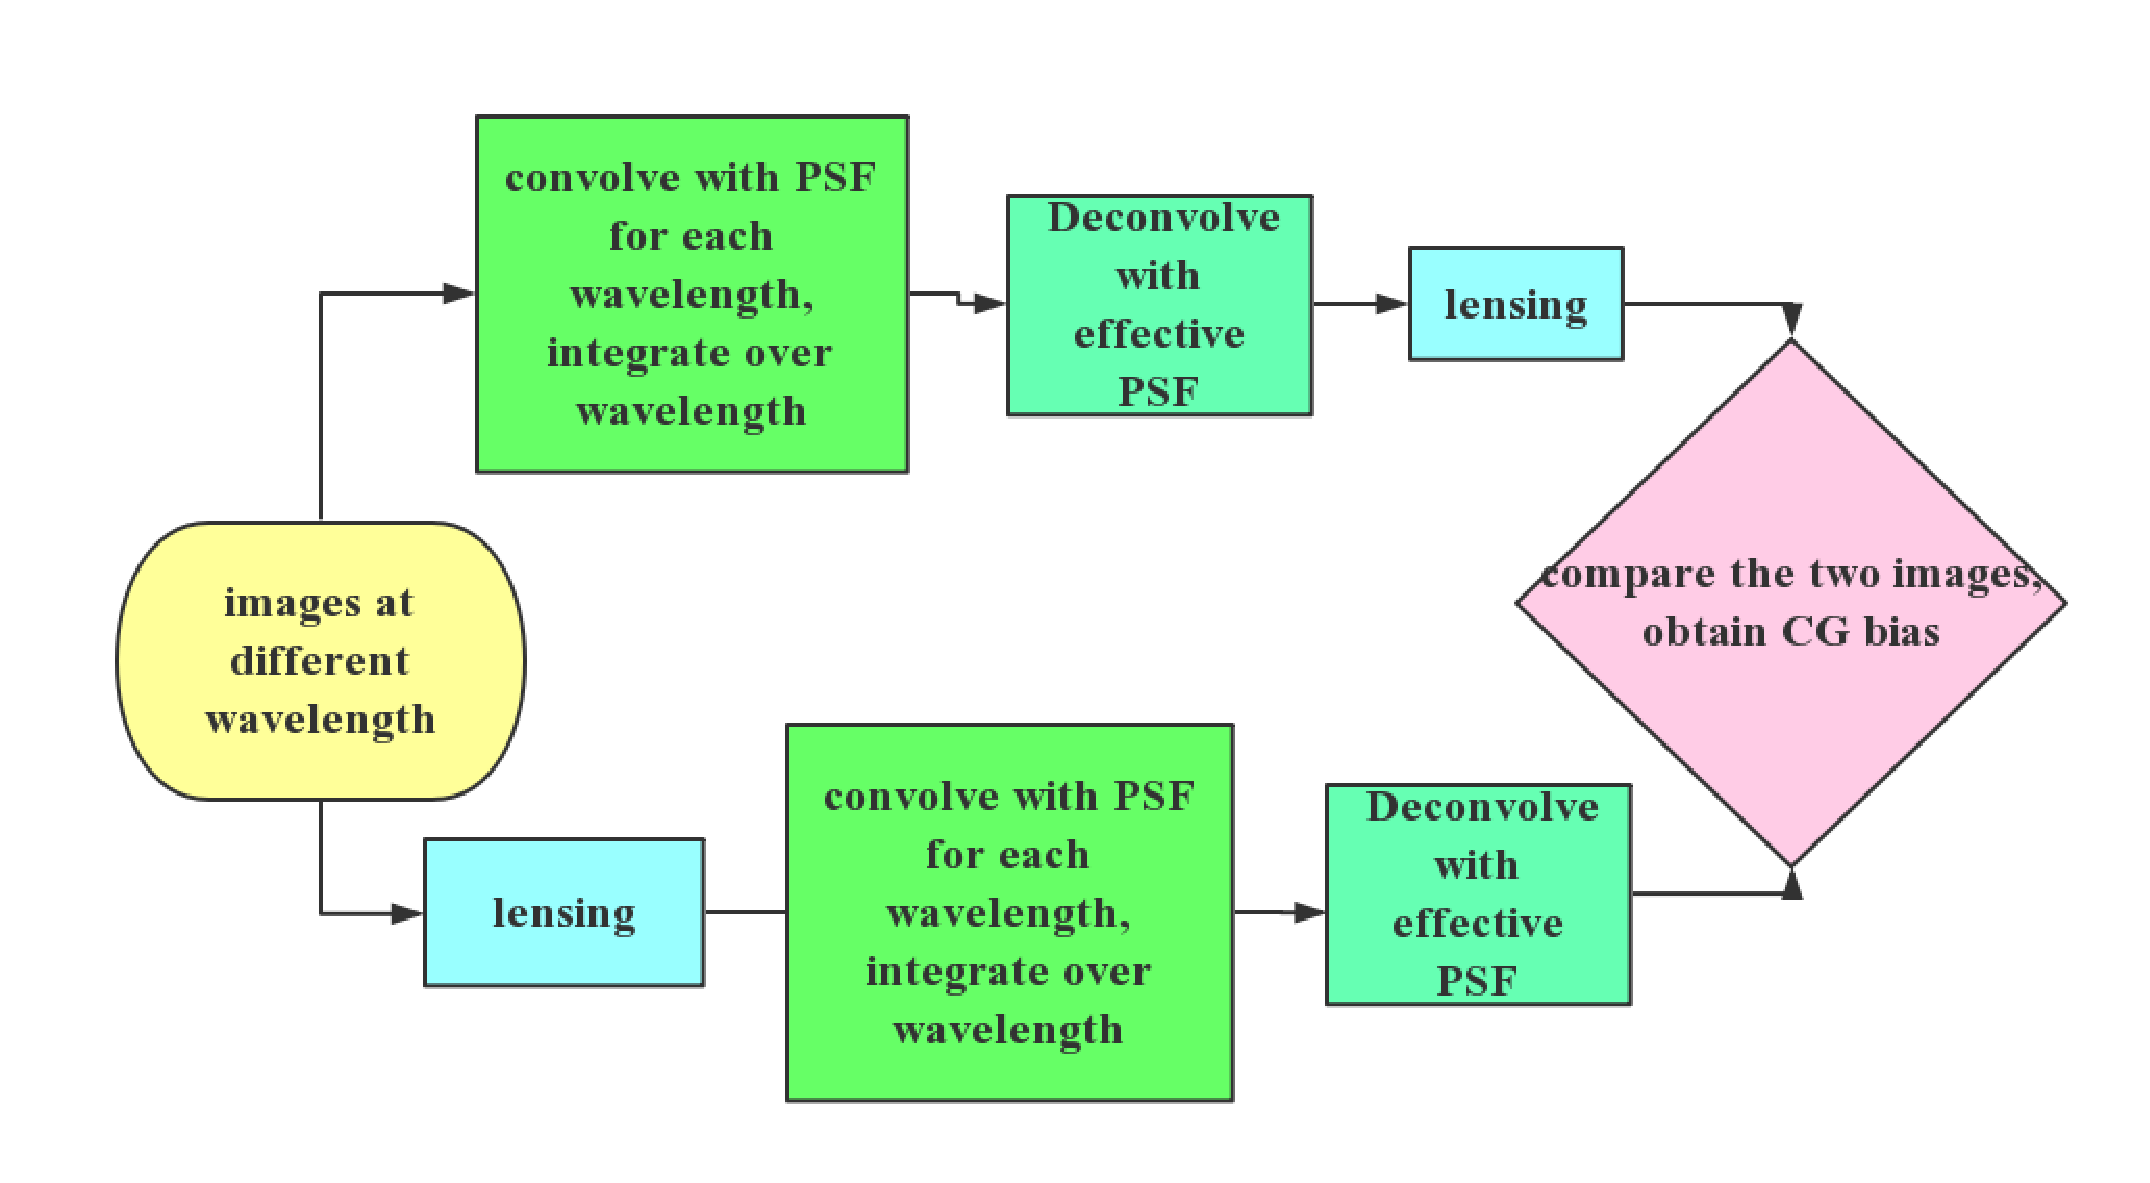
\includegraphics[width=12.5cm]{colourg.eps}
\caption{The steps of how we simulated CG (bottom flow) and NCG (top
  flow) images to estimate the shear CG bias.}
\label{fig:flowchart}
\end{figure*}
%

\section{Colour gradient bias in simulated data}

The CG bias is a higher order systematic bias, the numerical noise in
simulated images may cause extra error in our analysis. Thus, we first
adopt two independent codes to generate the simulated images: one is C/C++
and the other is python-based GalSim package
\citep{2015A&amp;C....10..121R}. In the C code, we directly calculate
the brightness density at the centre of each pixel, and sample the
image using the approximate brightness in each pixel (brightness at
the centre multiply the area of pixel). In GalSim the image are sampled
by FFT rendering.
%
The circular images are used for the source galaxy. We check the
initial mock image, especially the convolution and deconvolution 
step. No significant ellipticity are found in neither C or
GalSim.  Since the deconvolution is particularly difficult in the
numerical calculation, we also perform that for the elliptical
images. A small relative error $\sim10^{-6}$ appear in ellipticity
using both C and GalSim, which is two orders of magnitude smaller than
the possible CG bias.

We apply the two same galaxy models as in ES13. It will allow us to further
check the numerical error, since in ES13 the images are simulated by
different code. The images are consist of two
components: bulge and disk, both are modeled by a Sersic profile with index $n$
%
\be
I_{\rm Sersic}(\theta) = I_0 {\rm e}^{-\kappa\; \theta^{1/n}},
\ee
%
where $I_0$ is the central intensity, and $\kappa=1.9992\,n -
0.3271$.  For the SED of the bulge and the disk we use the galaxy
templates from \citet{1980ApJS...43..393C}. The SED of the bulge is
modeled by an elliptical galaxy, and SED of irregular galaxy for the
disk. We choose an extremely blue SED for disk to generate large
colour gradient in the galaxy images. For each wavelength, we
construct the galaxy image $I(\theta,\lambda)$ by adding up the
profiles of bulge and disk normalised by fixing the ratio
$S_{bulge}/S_{disk}$ at $\lambda=550$nm. The integrated profile is
applied to the Euclid filter in a wavelength range $[550:\,920]$nm
with a step of $1$nm. The images are constructed in an isolated stamp
with size $256\times256$ pixels, and resolution $0.05$ arcsec/pixel
(Table \ref{table:galaxy model}).

We use different reference PSF models. The first one is a Gaussian profile,
with wavelength dependent width:
%
\be
\sigma_{psf}(\lambda) = w_{0,800}\rund{\lambda \over 800{\rm nm}},
\elabel{psf}
\ee
%
where $w_{0,800}$ is the width of the PSF at $800$nm. In this section
we use $w_{0,800}=0.102$ arcsec, which is the same as in ES13. The
other reference model is an Airy function, which is close to the
Design profile \citep{2011arXiv1110.3193L}
%
\be
P(\theta) = {I_0 \over (1-\epsilon^2)^2} \rund{{2J_1(x)\over x} - {2\epsilon J_1(\epsilon x) \over x}}^2,
\elabel{psfairy}
\ee
%
where $I_0$ is the maximum intensity at the center, $\epsilon$ is the
aperture obscuration ratio, and $J_1(x)$ is the first kind of Bessel
function of order one. $x$ is defined as $x=\pi \theta/l$, where
$l=\lambda/D$ is wavelength over diameter ($\epsilon=1/3,\; D=1.2$ for
Euclid). In Fig.\,\ref{fig:psfmodel}, we compare the Airy model with
other PSF models.

%
\begin{table}
  \begin{tabular}{|l|l|}
    \hline\hline
    PSF  &Description\\
    \hline
    Gaussian &Gaussian PSF described by Eq.\,\ref{eq:psf} with $w_{0,800}=0.102$\\
    \hline
    GaussianT &Gaussian core described by Eq.\,\ref{eq:psf} with $w_{0,800}=0.054$\\
    &plusing top-hat with 20 percent of the total flux\\
    &the cut-off size $\propto\lambda^{0.74} (ES13)$\\
    \hline
    Airy  &Airy model with obscuration $1/3$ (Eq.\ref{eq:psfairy})\\
    \hline
  \end{tabular}
  \caption{\label{table:psfmodel}The PSF models shown in
    Fig.\,\ref{fig:psfmodel}.  The Gaussian model, which is the same
    PSF model in ES13 is used for the simulated images.  The GaussianT
    model is a Gaussian core plus a top hat function (ES13), which is
    shown as a comparison with Airy model.  The Airy model is used for
    the bias calibration and HST data analysis in the following
    section.}
\end{table}
%
\begin{figure}
\centerline{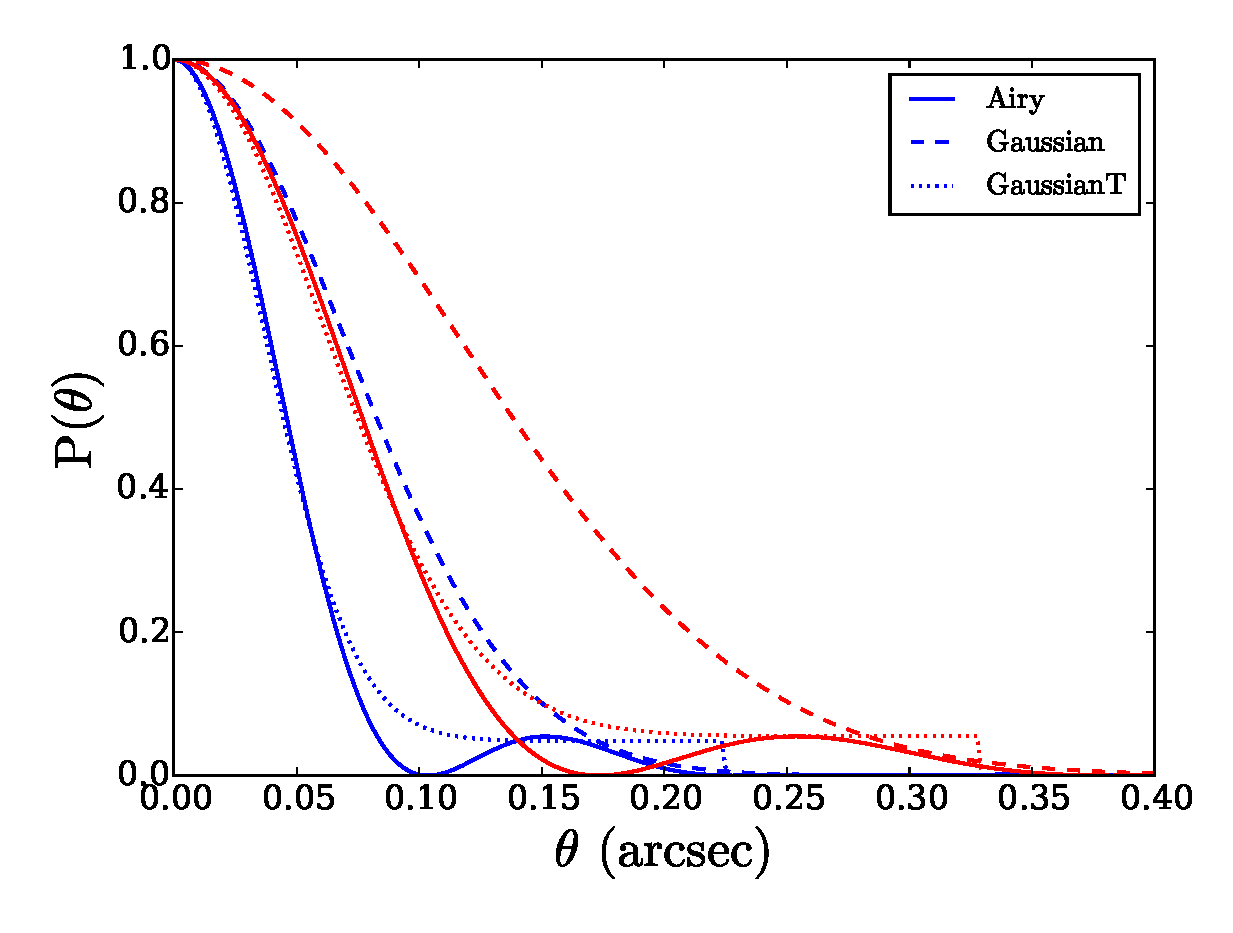
\includegraphics[width=6.0cm]{zairy.eps}}
\caption{Comparison of the PSF models at $550$nm (blue) and $920$nm
  (red): the solid, dashed and dotted lines are the Airy, Gaussian and
  GaussianT PSF models respectively (Table \ref{table:psfmodel}).}
\label{fig:psfmodel}
\end{figure}
%


%
\begin{center}
\begin{table}
\begin{tabular}{|c|c|c|c|c|}
\hline\hline
Name  &SED  &axis(arcsec) &flux ratio (550nm)  &Sersic index $n$ \\
B-galaxy  &E/Irr &0.17/1.2  &1:3  &1.5/1.0 \\
S-galaxy  &E/Irr &0.09/0.6  &1:3  &1.5/1.0 \\
\hline
\end{tabular}
\caption{\label{table:galaxy model} Parameters of simulated galaxies:
  when two values are quoted in a column, the first refers to the
  bulge, the second to the disc.}
\end{table}
\end{center}
%

We measure the CG bias as a function of weight size
(Fig.\ref{fig:biasofweight}). The solid lines are the results from
ES13, and the dashed (dotted) lines are the results using C (GalSim)
code. The blue and green lines are the CG bias of small size galaxy
(S-galaxy), while the red and purple lines are that of big size galaxy
(B-galaxy). One can see that the CG bias from all three different
simulated galaxies are consistent, i.e. the numerical error does not
introduce significant bias in this study. Thus, in the following of
this section, we will only use the GalSim to generate the mock
galaxies.
%
The CG bias decreases with the increasing weight size.  As the optimal
choice to maximize the signal-to-noise ratio is to match the weight
function to the size of the source galaxy, we will use the half light
radius for the weight function in the following of this paper. For the
two mock galaxies, the CG bias with such a weight function is
$0.8\times10^{-3}, 2\times10^{-3}$ for B- and S-galaxy respectively.
The smaller size galaxies have a larger CG bias, which suggests that
the calibration of the CG bias need to take into account of the size
as well as the real colour gradient of the galaxy.
%(the reason for the small divergence of blue lines is that the
%parameters used for simulating galaxy are slightly different).

Besides shear, there are higher order image distortions in weak lensing,
such as flexion \citep[e.g.][]{2002ApJ...564...65G,bacon2006}. In
previous analysis, we only consider the shear effect in the lensing
process, while the higher order image distortions also suffer from CG
bias as well. In additional tests, we perform the complete lens
ray-tracing instead of solely shearing the images. (We only use our C
code in this part, since the current version of GalSim only provides
shear effect.) We adopt an Singular Isothermal Sphere halo model as
the lens model, and vary the configuration within some reasonable
range, such as the Einstein radius, and the separation between the
lens and the source image (the corresponding shear value varies
between about $[0.02, 0.1]$). We find that the variation of lensing
magnitude can cause different CG bias (yellow shadow in
Fig.\ref{fig:biasofweight}), and in most time the flexion effect will
increase the CG bias. Such effects do not appear if we solely shear
the images. However in general case, the cosmic shear has a value
about a few percents. We can see that from the bottom boundary of the
yellow shadow, the bias are almost the same as that only considering
the shear effect. Only in case of the galaxy cluster lensing,
galaxy-galaxy lensing, especially in the strong lensing region, when
the flexion becomes significant, one has to take into account of such
kind of effect.


%
\begin{figure}
\centerline{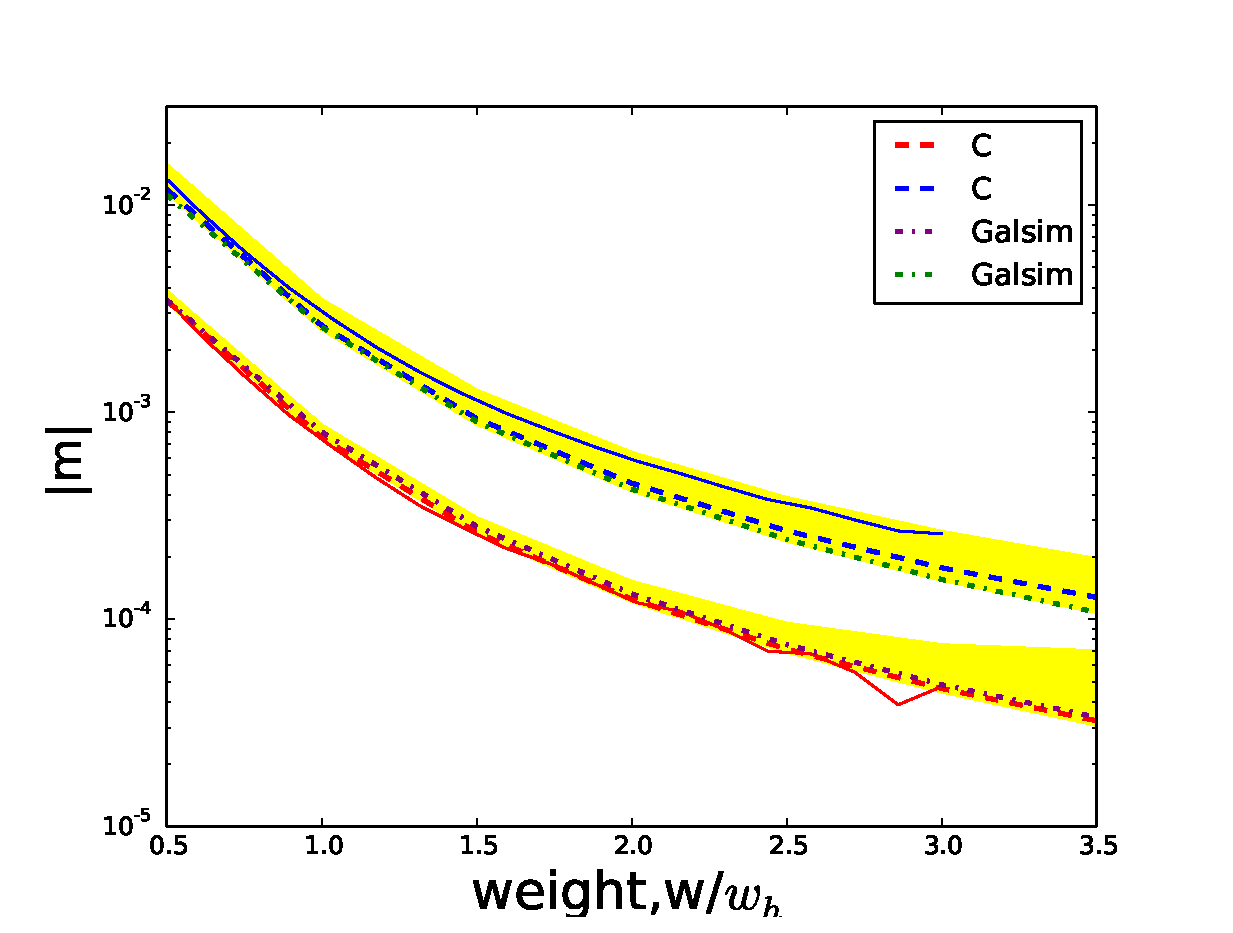
\includegraphics[width=8.0cm]{cvsgalsim.eps}}
\caption{The CG bias in shear versus weight function.  The
  solid lines are the results from paper ES13. The dashed
  (dash-dotted) lines are the results of this work using images
  simulated from C (GalSim) code. The blue (red) lines are the result
  for small (big) size simulated galaxies. The yellow shadow is the
  variation introduced by higher order image distortions. $w_h$ is
  half light radius of the galaxy image.}
\label{fig:biasofweight}
\end{figure}
%\begin{figure}
%\centerline{\includegraphics[width=12.0cm]{cgalsimz.eps}}
%\caption{The bias due to colour gradient as a function of redshift.}
%\end{figure}
%\begin{figure}
%\centerline{\includegraphics[width=10.0cm]{cfig6.eps}}
%\caption{Reproducing Fig.6 in ES13}
%\end{figure}
%\begin{figure}
%\centerline{\includegraphics[width=8.0cm]{c2bandB.eps}
%\includegraphics[width=8.0cm]{c2bandS.eps}}
%\caption{Estimaiton of CG bias using two band HST images. }
%\end{figure}

\subsection{Calibration of CG bias using simulated HST images}

We outline the method that calibrate the CG bias using two bands
images, while the details can be found in ES13. We will use two narrow
band images to reconstruct the image at each wavelength. For each of
the narrow filter the image can be approximated by:
%
\be
I_i(\theta) = \int_{\Delta \lambda_i} T_i(\lambda)\, I(\theta,\lambda) \;\d \lambda,
\elabel{linearitp}
\ee
%
where $T(\lambda)$ is the transmission, and $i=1,2$ stand for the two bands.
We assume that for each pixel the image can be interpolated linearly:
%
\be
I(\theta,\lambda) \approx
I_{\rm inter}(\theta,\lambda)=a(\theta)\lambda + b(\theta).
\elabel{interpolate}
\ee
%
Eqs.\ref{eq:linearitp} and \ref{eq:interpolate} yield a linear set of
equations on each pixel, which can be used to solved for the
coefficients $(a,b)$:
%
\be
T_{ai} \lambda a(\theta) \,+\,T_{bi} b(\theta) = I_i(\theta), \quad\; i=1,2,
\elabel{lineareq}
\ee
%
where $T_{ai,\,bi}$ is the integrated transmission function at two
filters. With $(a,b)$ and Eq.\ref{eq:interpolate}, one can obtain
approximated galaxy images of each wavelength
$I(\theta,\lambda)$. Then we will follow the same procedure as in
previous section to estimate the CG bias.

The same two galaxy models from previous section are used in the
simulation, and we simulate the images in two HST filters: F606W,
F814W, which cover the filter of Euclid image survey. The spectra of
the galaxy are shifted according to their redshift, but the evolution
of the galaxy or the cosmology are not adopted in the simulation. The
spatial resolution is $0.05$ arcsec/pixel. The PSF is modeled by the
Airy function with diameter $D=2.5$ and obscuration $0.33$, which is
the configuration of HST. As shown in ES13, one needs to correct the
PSF effect in the observed images, or the CG bias will be
underestimated. We will adopt the same step: deconvolution for images
before the bias estimation and discuss that for the noisy images
later.

In order to see the effect of noise in the galaxy image, we add
Gaussian noise into the simulated HST images. An ideal level (SNR=50)
and a moderate level (SNR=15) are used to see the effect of the CG
bias. The RMS of the Gaussian image noise is determined by the total
flux ($F_{tot}$) within a certain radius $1.5\,r_h$
%
\be
\sigma = {F_{tot} \over {\rm SNR} \sqrt{N_{tot}} },
\ee
%
where $N_{tot}$ is the total pixel number within $1.5\,r_h$.  In
Fig.\ref{fig:ests2n}, we compare the input SNR with that estimated by
SExtractor \citep{1996A&AS..117..393B}. We can see that the
estimations are slightly higher than the input values at $SNR=15$, but
still within a reasonable value for real weak lensing survey.
%
\begin{figure}
\centerline{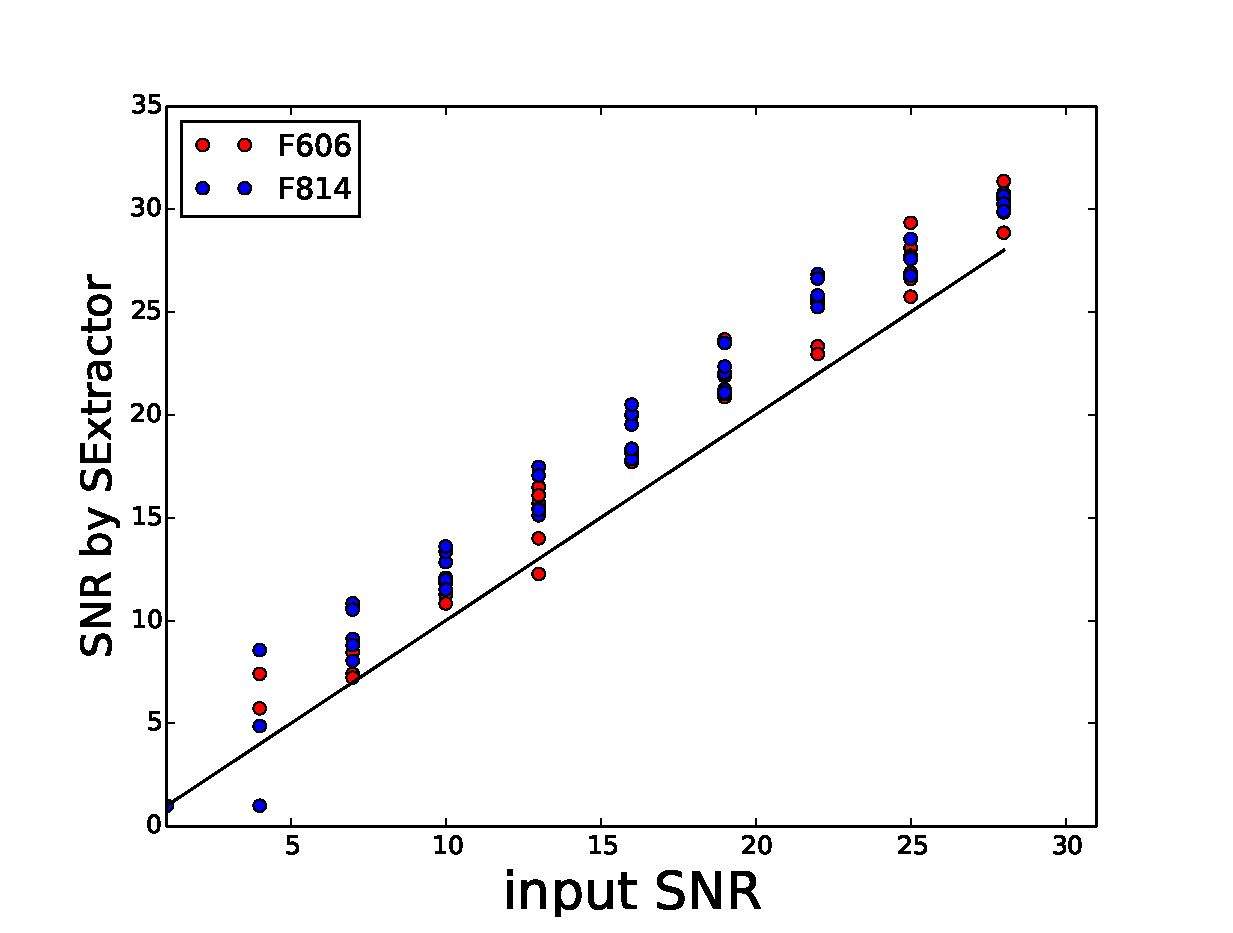
\includegraphics[height=5cm,width=5.0cm]{zs2ncB.eps}
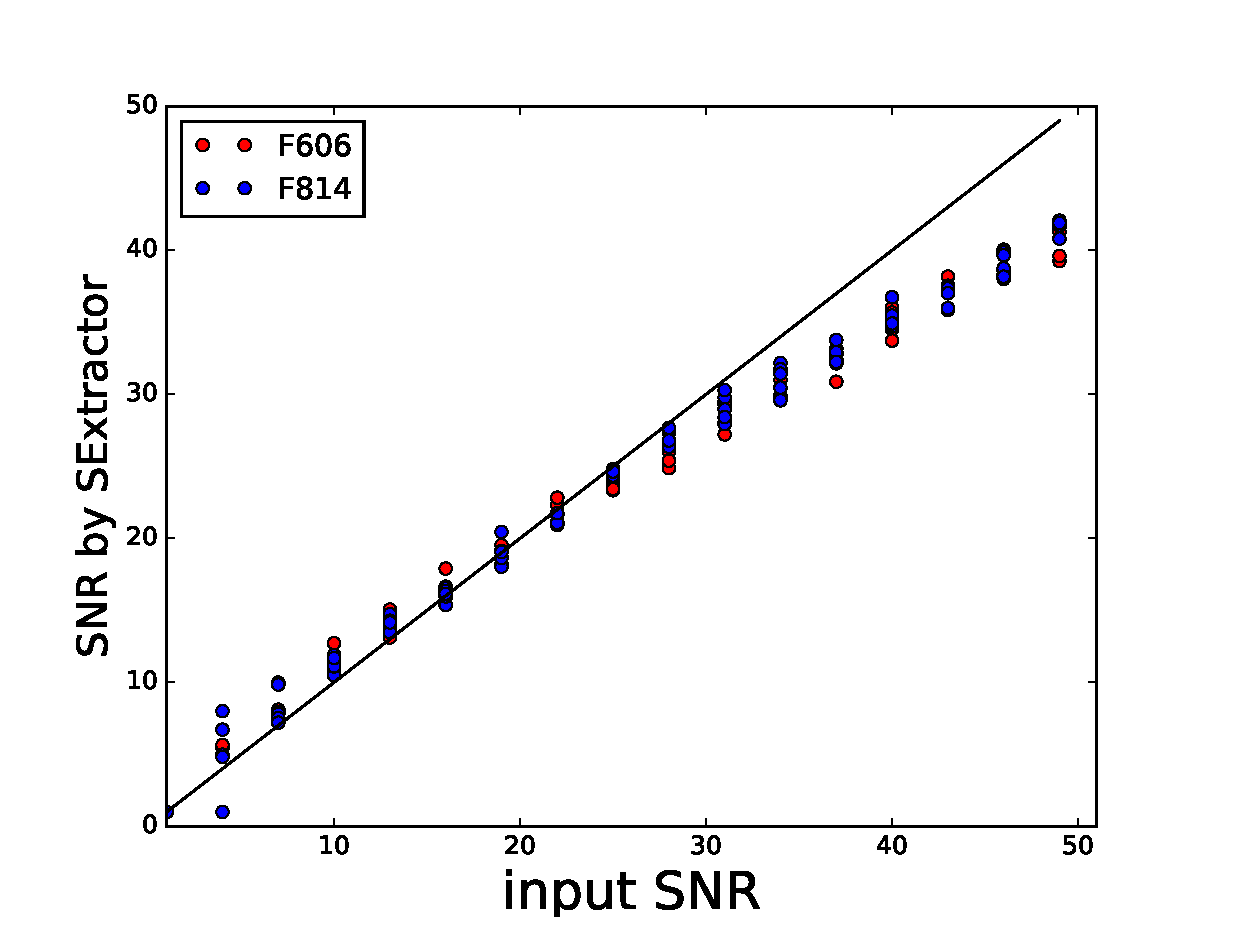
\includegraphics[height=5cm,width=5.0cm]{zs2ncS.eps}}
\caption{SNR estimated by SExtractor vs input SNR. Left is for the
  B-galaxy; Right is for the S-galaxy.}
\label{fig:ests2n}
\end{figure}
%

Direct devonvolution of a noisy image will end with a strange galaxy
image and large numerical noise, thus we apply Galfit
\citep{2010AJ....139.2097P} to fit the noisy image, and use the fitted
image as our noise reduced observed image, i.e. the residual noise is
not taken into account for CG analysis. For the necessary fitting
profile and number of components, we also use two Sersic components as
bulge and disk for both image bands. For each image, we apply further
constraints to the galaxy parameters: Sersic index, effective radius,
and axis ratio (Table \ref{fitpar}). We also compare with the input
models, and find that the Sersic index is more difficult to fit than
the effective radius.
%the effective radius can be achieved at a small variations (within
%$20\%$), while the Sersic index usually has a large difference from
%the input values as well as scatter.

In order to provide a initial parameters for Galfit, we use the
stacked image of two bands to estimate the center and some initial
values of the galaxy parameters from SExtractor. The fitting images
slightly depend on the initial values, and can effect the estimate for
the CG bias estimation.  The dependence will become significant with
the decreasing of image SNR.  In the following estimation for the CG
bias, we will perform the image fitting using two kinds of initial
parameters: in the first one we will leave all the fitting parameters
free; while in the other one we will freeze the Sersic index as the
simulated value, and leave the others free. As we will present,
with sufficient large samples, the estimation using noisy images for the
CG bias can converge, and is independent of the initial parameters.

%
\begin{center}
\begin{table}
\begin{tabular}{|c|c|c|c|c|}
\hline\hline
 &S-606W  & S-814W  & B-606W & B-814W \\ \hline
$n_1$ &0.5-2.5  &0.5-2.5  &0.5-2.5 &0.5-2.5 \\ \hline
$n_2$ &0.5-2.5  &0.5-2.5  &0.5-2.5 &0.5-2.5 \\ \hline
$R_{bulge}$ &1-10 &1-10  &3-30  &3-30  \\ \hline
$R_{disk}$  &5-30 &5-30  &10-60 &10-60 \\ \hline
$q$      &0.6-1  &0.6-1  &0.6-1 &0.6-1 \\ \hline
\hline
\end{tabular}
\caption{\label{fitpar} Constraints for the fitting parameters in Galfit.
The first two columns are for two images of the S-galaxy, the other two are
the image of B-galaxy.
$n_1$ is the Sersic index for bulge, and $n_2$ is the Sersic index for disk.
The effect radius is given in unit of pixel ($0.05$ arcsec).}
\end{table}
\end{center}
%
%\begin{figure}
%\centerline{\includegraphics[width=7.0cm]{zsnrre.eps}
%\includegraphics[width=7.0cm]{zsnrn.eps}}
%\caption{The fitting parameters (Sersic index and effect radius).}
%\end{figure}

Applying the calibration method to the fitted images, we can obtain
the estimation of the CG bias for the simulated images. In
Figs.\ref{fig:biasofz50} and \ref{fig:biasofz15}, we show the shear CG
bias with redshift. In each panel, we show different estimates for the
bias: 
\begin{itemize}
\item
The black solid lines are the ``True'' CG bias: we use the true
SED of the galaxy and images of each wavelength to estimate the bias
without approximation. 
\item
The dashed lines are the estimation using two
HST images without noise.
\item
The colour lines are those using noisy
images. The difference between red and blue lines are in the step of
Galfit: for the red lines, we free all the parameters in image
fitting, for blue lines we fix the Sersic index as the input
value. For the orange lines we also free all the parameters, but we
perform another convolution with the effective PSF (see appendix for
more detail). In Fig.\ref{fig:flowchart} one can see that the
convolution is canceled with the last deconvolution for the CG images.
The reason for that is the deconvolution may cause some numerical
errors, especially for the small size noisy images. The extra PSF
convolution will not significantly change the CG bias as we will show
in the appendix. Therefore, in the following result for noise images,
we will perform the convolution to the NCG image instead of
deconvolution to the CG one.
\end{itemize}
Moreover, although we use the circular source image in the simulation,
the fitted noisy images will become slightly elliptical. In order to
get rid of the error due to the ``intrinsic shape'', we rotate the
source image $6$ times, and use the average value as our estimate for
the galaxy ellipticity \citep{2007AJ....133.1763N}. At each redshift,
we use one noise free image and $40 (200+)$ noisy images for $SNR=50
(SNR=15)$.  In the bottom panel of each figure, we also show the
residues with respect to the true CG bias, and the error bars, which
are given by the standard deviation from $e_{cg}$ and $e_{ncg}$
%
\be
\sigma_m= |m| \sqrt{\rund{\sigma_{cg} \over \langle e_{cg}\rangle }^2
  + \rund{\sigma_{ncg} \over \langle e_{ncg} \rangle}^2 }.
\elabel{sigmam}
\ee
%
In the error panel, the grey shadow stands for the error budget of CG bias in
Euclid cosmic shear analysis \citep[$\pm
  0.00025$][]{2013MNRAS.431.3103C,2013MNRAS.429..661M}.

One can see that in general our estimate can reproduce the properties of CG bias
in ellipticity measurement using both ideal or noisy images.
In the high SNR cases (Fig.\ref{fig:biasofz50}), all the estimates with different
initial parameters basically agree with each other, and reproduce the
properties of the CG bias as a function of redshift. The estimate with
all fitting parameters free gives lower bias than that fixed the Sersic index.
In the realistic SNR case (Fig.\ref{fig:biasofz15}),
the fitting using all free parameters show better estimates for the CG
bias, and the errors are within the requirement for most cases.
The variance due to the image fitting with different initial parameters
are larger than high SNR cases, but can still be reduced by large sample
of images and reach the requirement. Therefore, for each type of galaxy,
at one redshift, we need at least $300$ galaxy images for calibrating the
bias. The scatters in the estimation are proportional to the magnitude of the
bias, i.e. we have large uncertainty for S-galaxy at low redshift.
%%%%%%%%%%%%%%%%%%%%%%% PSF corrections
In additional tests using other measurement methods for PSF
correction, such as the image fitting methods
\citep[e.g.][]{2007MNRAS.382..315M,2008MNRAS.390..149K,2013MNRAS.429.2858M},
and KSB+ \citep[e.g.][]{1998ApJ...504..636H,2006MNRAS.368.1323H}, we
find that the bias has similar dependence on the SED of the galaxies,
although the magnitudes are different.

In all estimates, both low and high SNR, we notice that at $z=0.5$ and $0.9$, the estimates are
significantly smaller than the true value for both galaxy models. This is
due to the uneven SED of the source galaxy in the two HST filter. In
Fig.\ref{fig:sedz}, we compare the SED of the galaxy in redshift
$z=0,0.5$. One can see that at $z=0.5$, besides the strong emission
lines, the linear approximation cannot reflect the properties of the
source galaxies. Thus for the galaxies with strong emission lines, two
wide band images are certainly not sufficient to calibrate the CG bias.
%In Fig.\ref{fig:err2snr}, we show the average residual bias
%$\bar{|m|}$ over the redshift as a function of SNR of the images. For
%each SNR, we average the residual in redshift range from $0$ to $1.2$,
%and for each redshift, $50$ noise realizations are used. One can see
%that for the images with SNR smaller than $\sim10$, the errors of our
%estimate will be non negligible, and the estimation thus cannot
%provide trustable calibration. Another simplification that we adopt
%here is that the SNR we used in two bands are the same. This is in
%reality not the case in most the time. In the more sophisticated
%simulation, the image SNR of two bands need to be determined by the
%colour of the galaxy.

%%%%%
\begin{figure}
  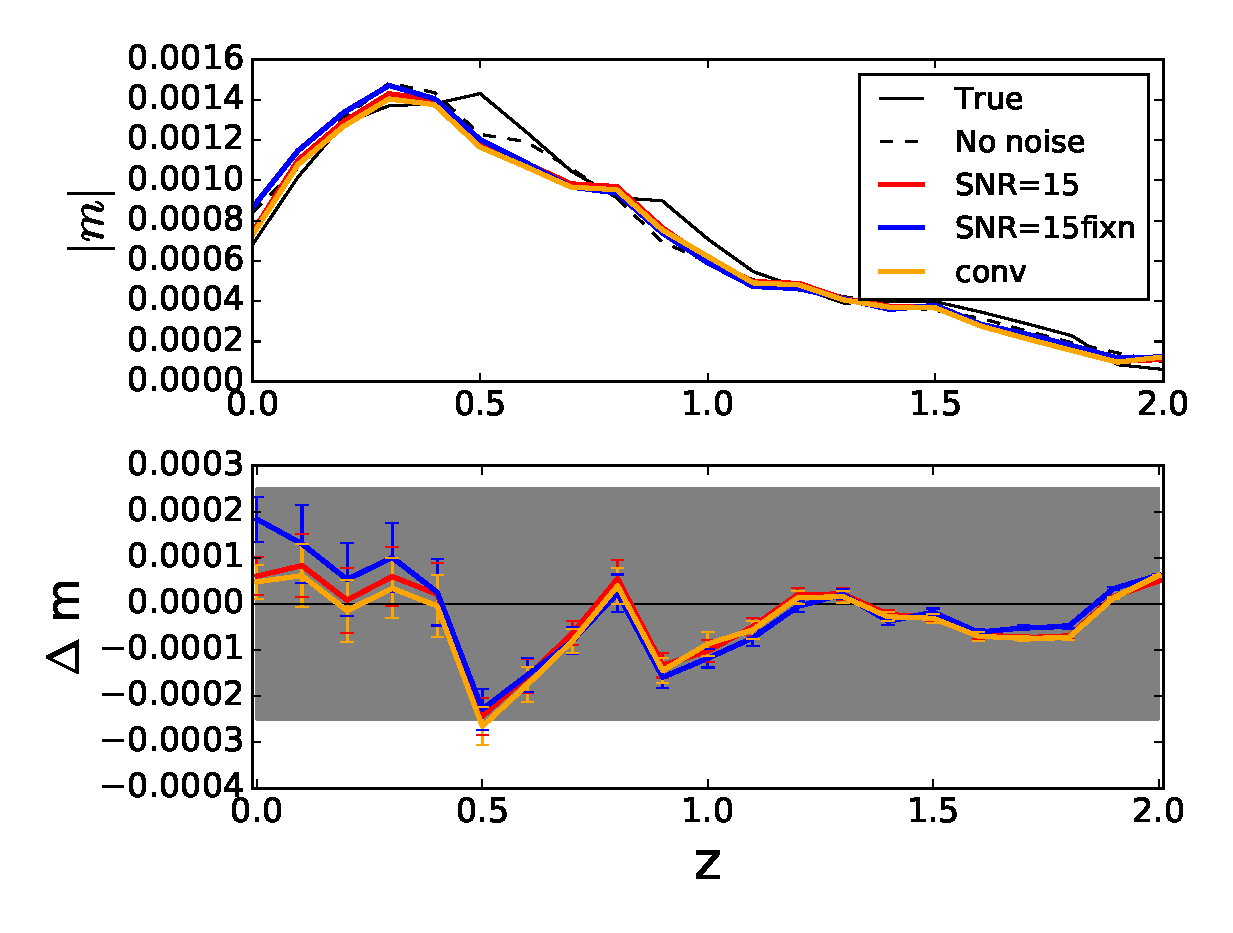
\includegraphics[width=8.0cm]{zs2n_b_snrtt50.eps}
  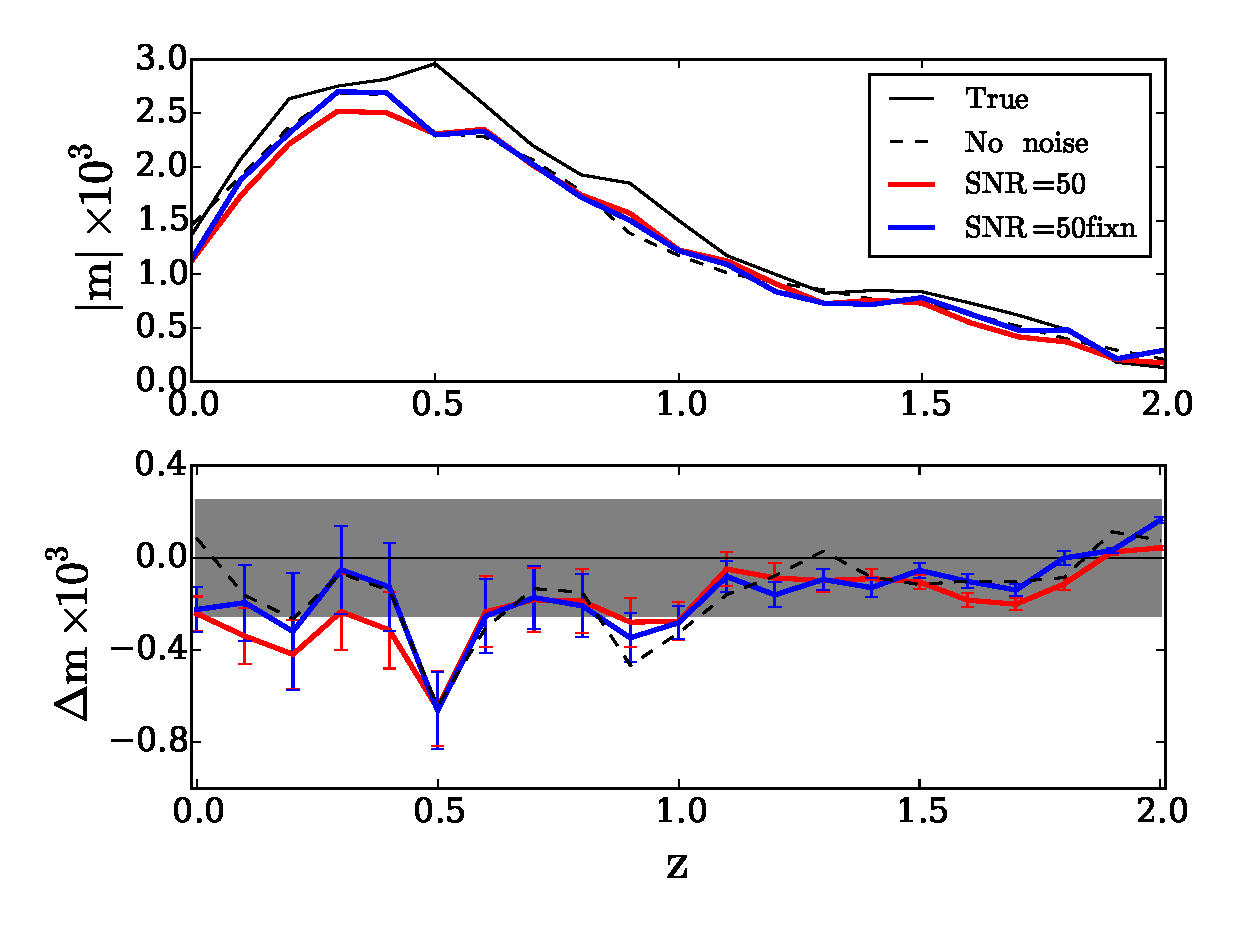
\includegraphics[width=8.0cm]{zs2n_s_snrtt50.eps}
\caption{The CG bias in shear measurement as a function of redshift
  using simulated images. The black solid lines are the true CG bias;
  the dashed lines are the estimation using two band HST images
  without noise; the colour lines are the estimation using noisy
  images of input $SNR=50$, the value are the average over $40$
  realizations each redshift. In the bottom, $\Delta m$ is the
  residual with respect to the true CG bias, and the error bars show
  the standard variations (Eq.\ref{eq:sigmam}). $Up(Down)$-figure are
  the results for B-(S-)galaxy.}
\label{fig:biasofz50}
\end{figure}
\begin{figure}
  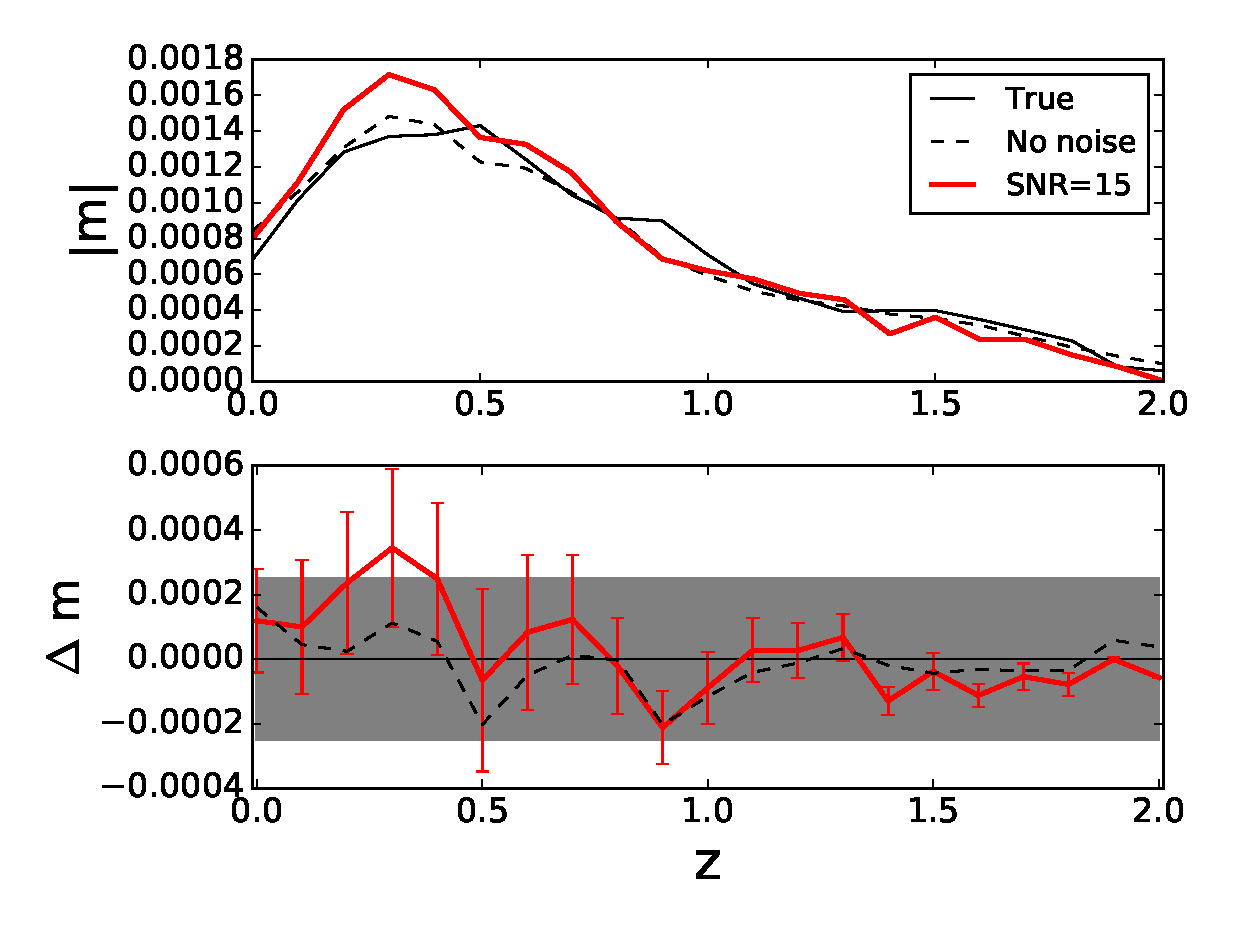
\includegraphics[width=8.0cm]{zs2n_b_snrtt15.eps}
  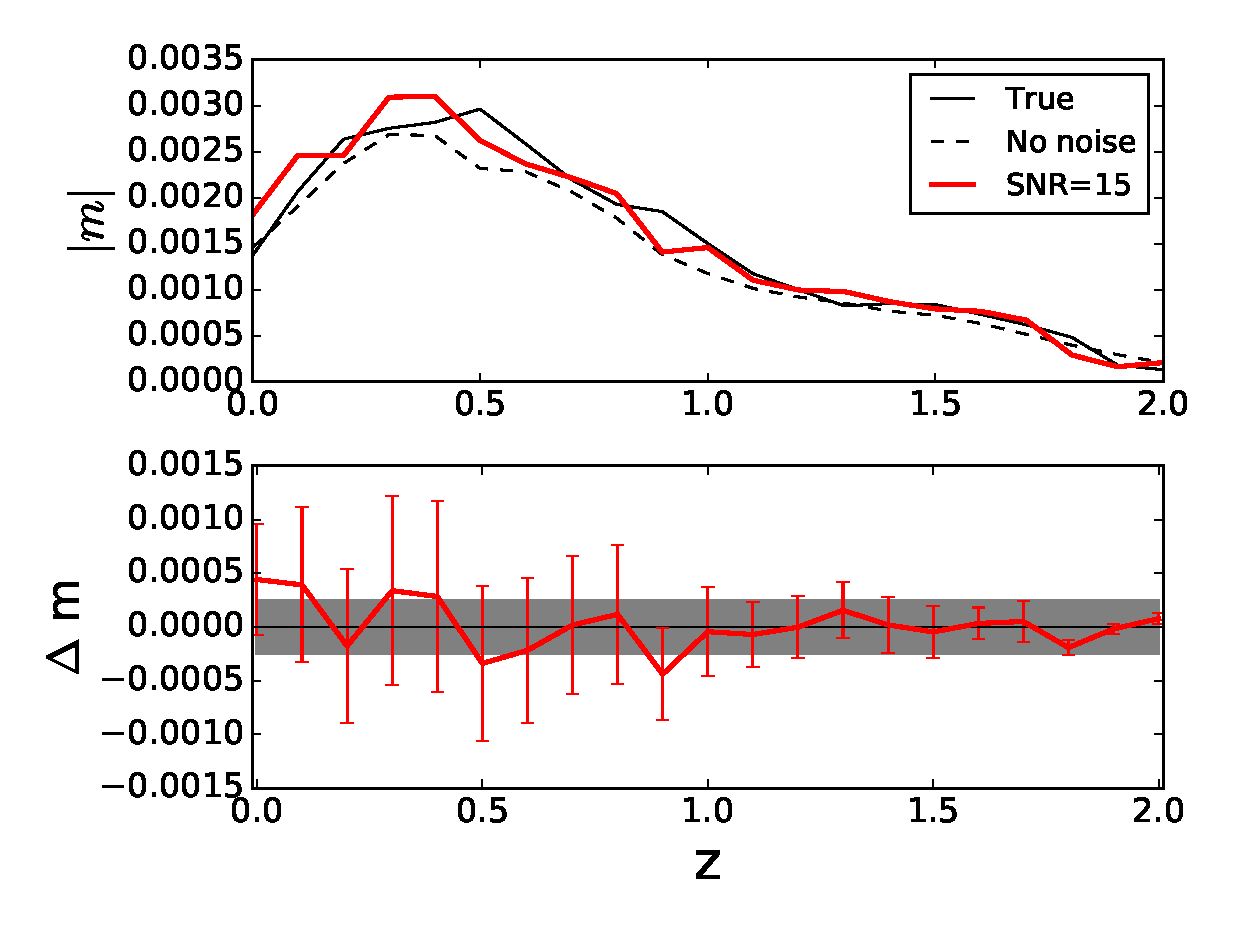
\includegraphics[width=8.0cm]{zs2n_s_snrtt15.eps}
\caption{Same as Fig.\ref{fig:biasofz50} but for images of SNR=15.
  $200$ realizations are used for the red lines at each redshift and
  $220$($320$) realizations are used for blues lines for the
  B-(S-)galaxy. }
\label{fig:biasofz15}
\end{figure}

%
\begin{figure}
\centerline{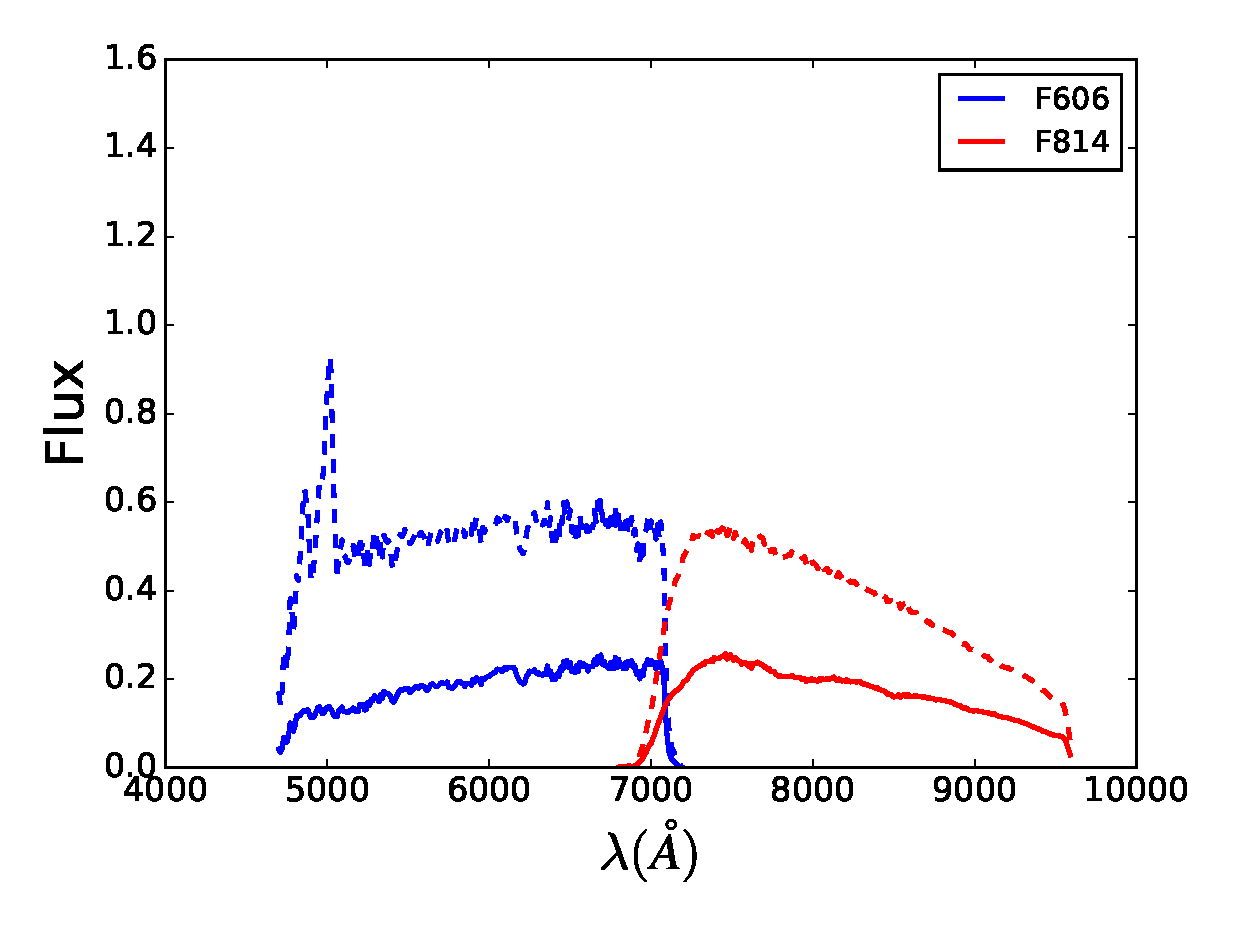
\includegraphics[width=4.0cm]{z0bandsed.eps}
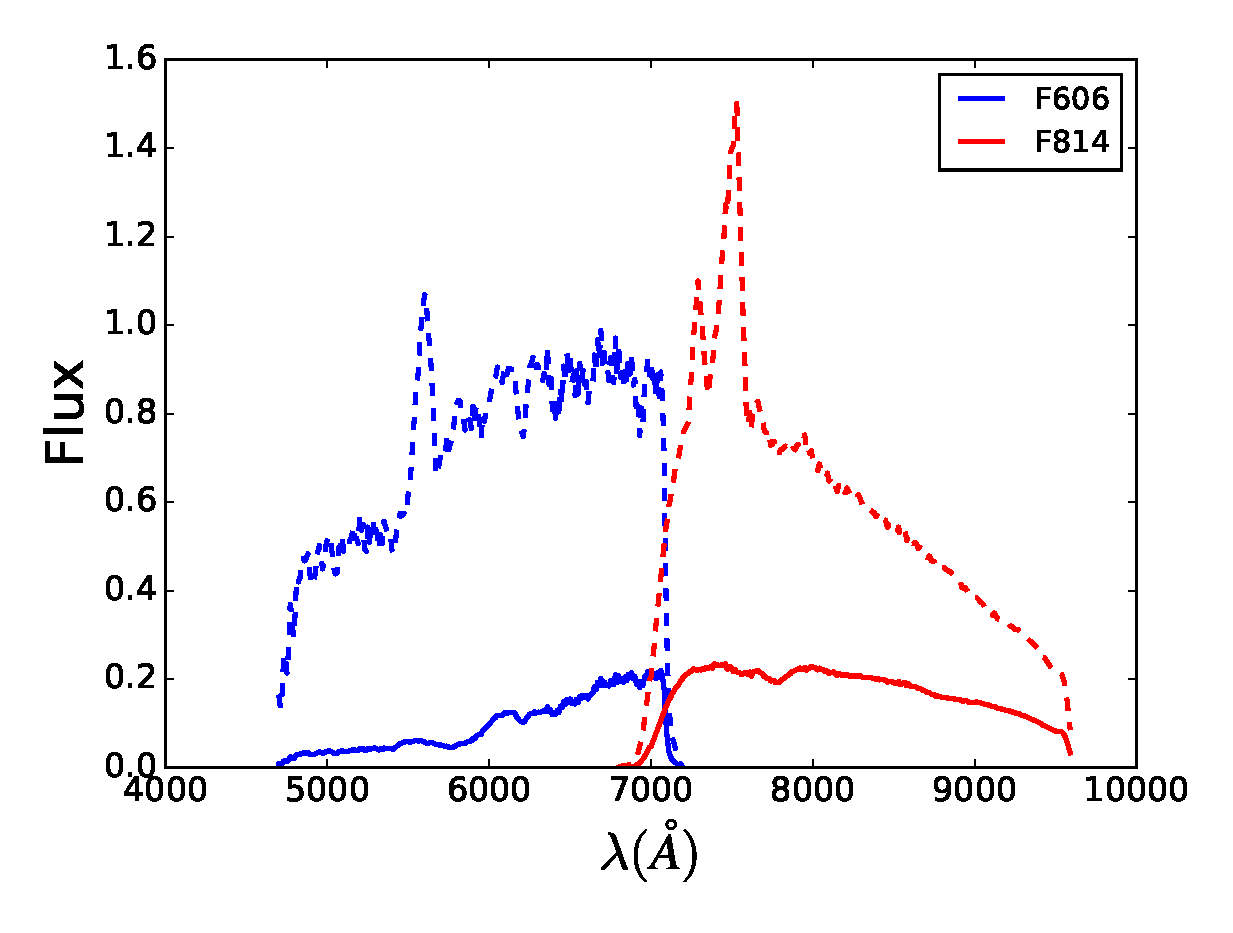
\includegraphics[width=4.0cm]{z5bandsed.eps}}
\caption{Spectral energy distributions used to create the disc and
  bulge components of our mock galaxies. They are normalized at
  $\lambda=5500$\AA$\,$ by ratio $F_{\rm bulge}/F_{\rm disk}=1/3$, and they
  are convolved with HST filter function in F606W and F814W. $left$-
  redshift $0$; $right$- redshift $0.5$.}
\label{fig:sedz}
\end{figure}


\subsection{PSF variations in calibration data from HST}

In the previous test, we used an ideal circular symmetric Airy PSF
model. It may however cause inaccuracy in our estimation of the CG
bias. Thus, we perform additional tests due to the variations of the
PSF. The noise free images are used in order to isolate the effects of
the PSF. The different PSF models are applied only in the step of
deconvolution for the simulated HST images.

First we generate three pairs of PSF model by slightly increasing the
size of PSF. The
effect on the CG bias is shown in Fig.\ref{fig:psfacc1}. From solid,
dashed to dotted lines, we increased the PSF size of the F606 bands; while
from red, green to blue lines, we increase the PSF size of the F814
bands. Although the effect due to the two PSF variations depends on the
SED of the source galaxy, one can see that increasing the size of the
PSF in different bands will cause either on increase or
decrease in the CG bias calibration. Once again, we can see that
the small galaxies are more sensitive to the variation of PSF.

Moreover, we generate 3 different PSF models using TinyTim
\citep{2011SPIE.8127E..0JK}: the first one is a normal PSF without
defocus, the second one is a bit larger but still realistic PSF, which
is generated by changing the parameter defocus offset of secondary
mirror to the primary, the third one is simply transposing of the
first one.  In Fig.\ref{fig:psfacc2}, we do not find significant
effects with slight variations on the PSF. This may be because we used
the circular symmetric, noise free images in the tests. For real
galaxy noisy images, the PSF may cause slightly stronger effects. In
additional tests, we calculate circular averages of the three PSF
models, and find slightly different CG bias when using the second
model PSF, since it has slightly larger size. Thus, the limited
accuracy of the PSF model in HST data
will not be an important source of error in our study.

%
\begin{figure}
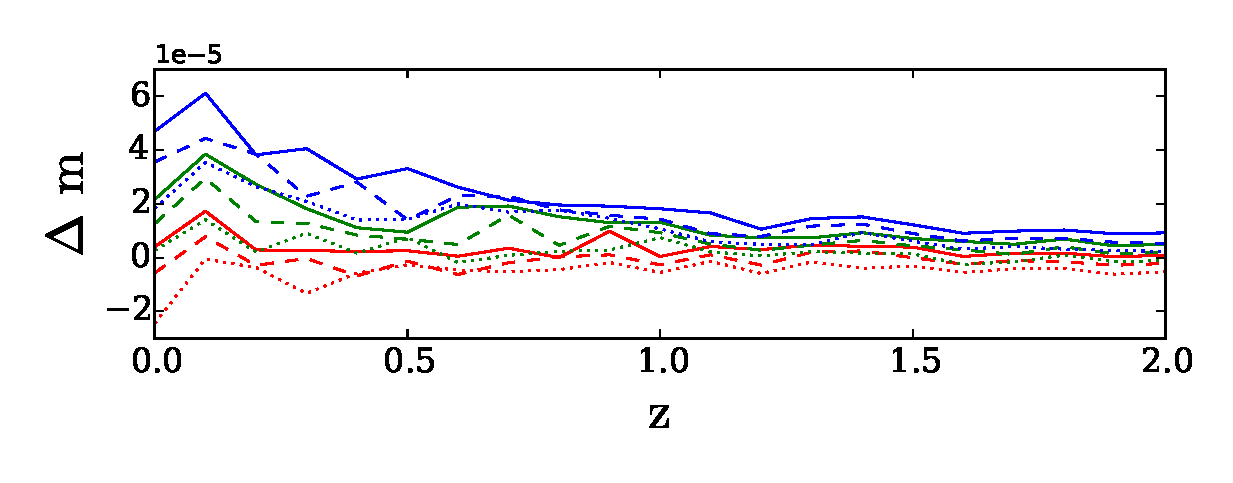
\includegraphics[width=8.0cm]{varpsfB.eps}
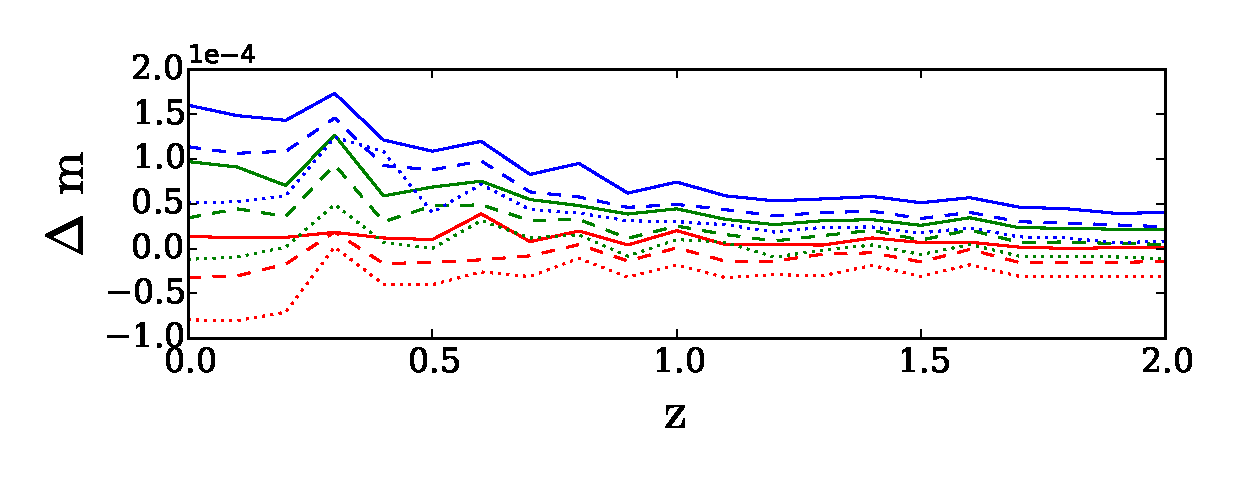
\includegraphics[width=8.0cm]{varpsfS.eps}
\caption{The PSF in the deconvolution are varied to see the effect on
  the CG bias.  From red, green to blue lines, we increase the size of
  PSF for the F814W; from the solid, dashed to dotted lines we
  increase the size of PSF for the F606W.  }
\label{fig:psfacc1}
\end{figure}
%
\begin{figure}
%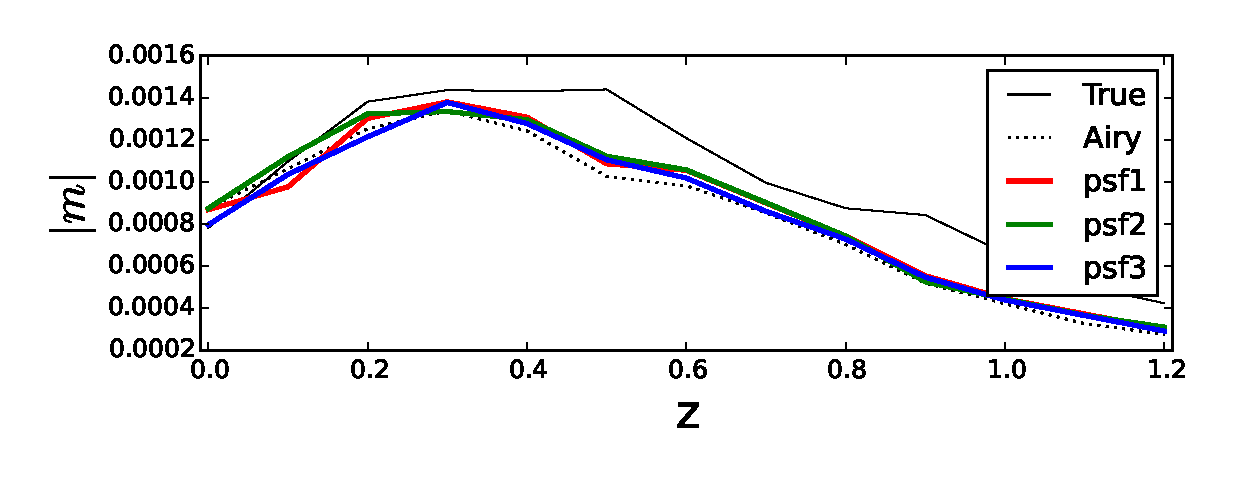
\includegraphics[width=8.0cm]{z_b_psfcomt.eps}
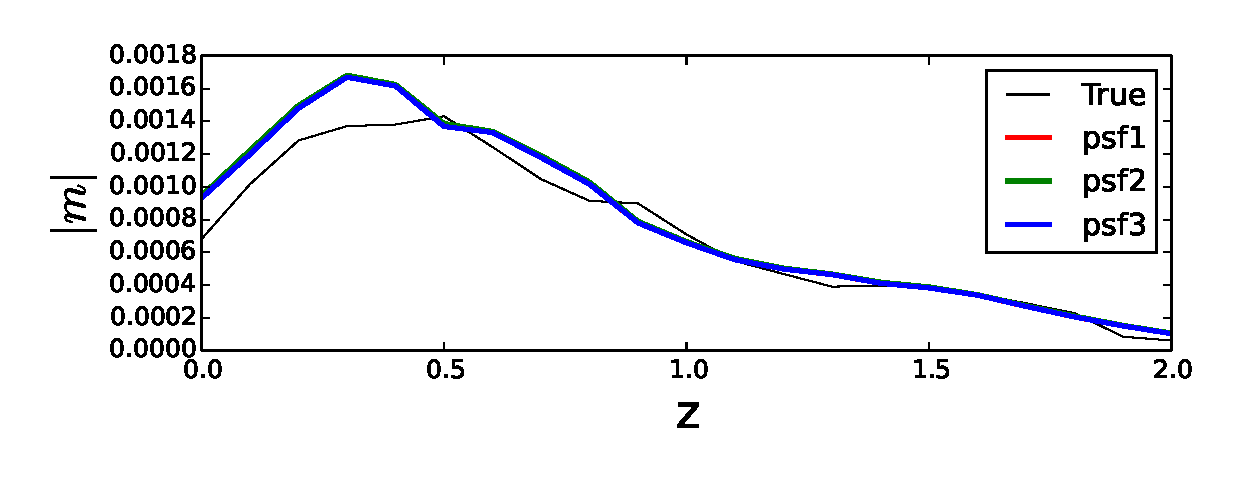
\includegraphics[width=8.0cm]{z_b_psfcom05.eps}
%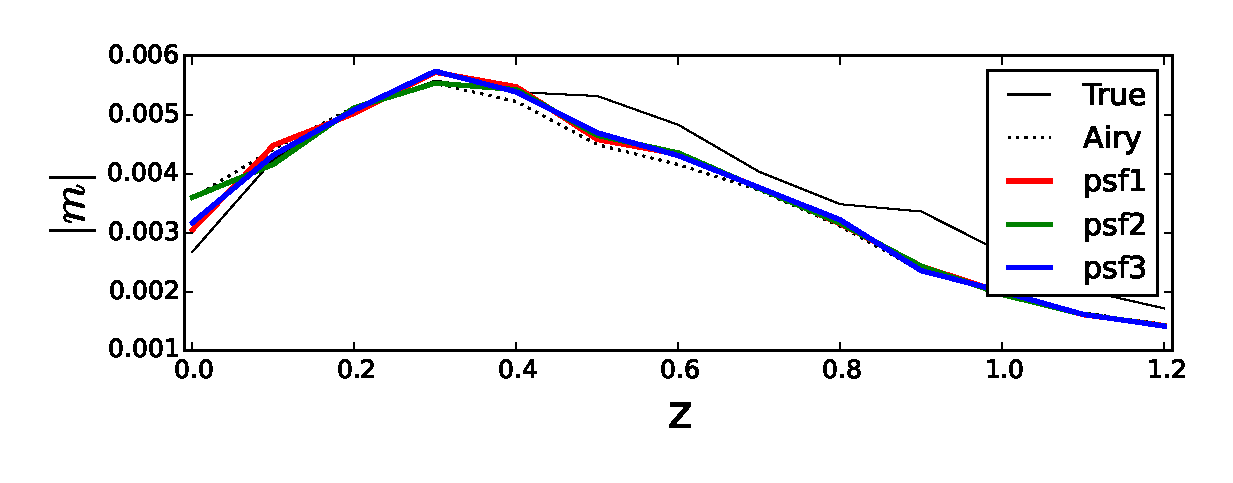
\includegraphics[width=8.0cm]{z_s_psfcomt.eps}
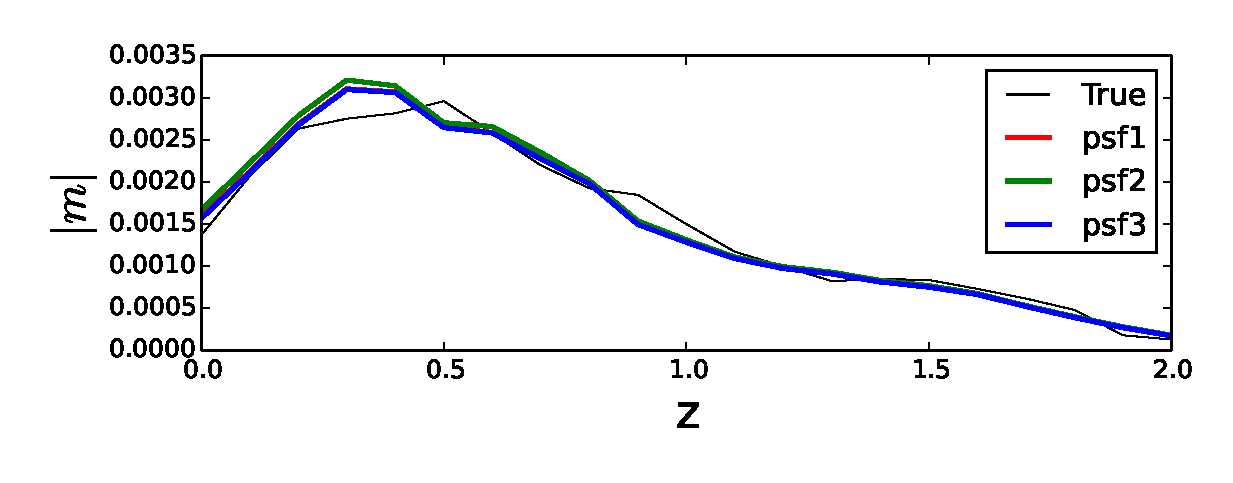
\includegraphics[width=8.0cm]{z_s_psfcom05.eps}
\caption{Same as Fig.\ref{fig:psfacc1} but using three different
  TinyTim PSF model. Top (Bottom) is for the B-galaxy (S-galaxy).}
\label{fig:psfacc2}
\end{figure}
%

\section{CANDELS data}

\subsection{Calibration sample}
In this section, we use the real galaxy images to estimate the CG bias
which will appear in the Euclid weak lensing survey. For the reference
PSF, we use the Airy model (Eq.\,\ref{eq:psfairy}).


To investigate the impact of colour gradients using realistic galaxies
populations, we employ HST/ACS data taken in the F606W and F814W
filters in the three CANDELS fields (AEGIS, COSMOS, and UDS), which have
a roughly homogeneous coverage in both bands
\citep[see][]{davis2007,grogin2011,koekemoer11}. We base our analysis
on a tile-wise reduction of the ACS data, incorporating pointings
which have at least four exposures to facilitate good cosmic ray
removal, yielding combined exposure times of 1.3-2.3ks in F606W and
2.1-3.0ks in F814W.  We employ the updated correction for
charge-transfer inefficiency from \cite{massey2014},
\texttt{MultiDrizzle} \citep{koekemoer2003} for the cosmic ray removal
and stacking, as well as careful shift refinement, optimised
weighting, and masking for stars and image artefacts as detailed in
\cite{schrabback2010}.  Schrabback et al. (in prep.) describe the
generation of weak lensing catalogues for these images.  We base our
analysis on the galaxies passing their source selection and apply
additional magnitude cuts as detailed below. To investigate the
dependence of the colour gradient influence on galaxy colour and
redshift, we match this galaxy catalogue to the photometric redshift
catalogue from \cite{skelton14}.  We list the total non-masked areas
in which these catalogues overlap in Table \ref{table:mag}.


We match the galaxy from V(F606W) and I(F814W) bands by selecting that
the difference of galaxy coordinates in two bands is smaller than 1
pixel ($0.05$ arcsec). Moreover, in order to resemble the Euclid image
survey, we apply selection based on the magnitude of two bands. In the
first selection, the galaxy must be brighter than magnitude $25$ in
V-band and $24.5$ in I-band. In the second selection (VIS, N2 sample),
we apply the linear interpolation from V and I band using the
effective wavelength to approximate the Euclid VIS magnitude, and
select the galaxy brighter than $24.5$ in VIS. In the last one (N3
sample), we enlarge the sample by using lower threshold in two bands:
$25.5$ in V and $25.0$ in I band. The amount of galaxies is listed in
Table\ref{table:mag}.
%
The galaxy VIS magnitudes will determined by several factors, such as
exposure time and filter transmission, etc. Thus, the actual number of
galaxies can be different from what we have shown in this work. The
approximation that we use rely on the flatness of the source
spectrum. In the VIS sample, the number of galaxies is similar to that in
the first selection in all three fields, which suggest that the
spectra of our galaxies are relatively smooth. In the N3 sample the galaxy
number is much higher.
%
The total galaxy number and number density ($\sim$12/arcmin$^2$) is
lower than that in ES13 for several reasons: the galaxies are selected
which the 3D-HST photometric redshift are available, and those
suitable for weak lensing analysis, e.g. the very big or bright
galaxies are not include. Moreover, in ES13 the galaxies are selected
by the magnitude of F814W. However we select galaxies by the estimated
VIS magnitude and well match in F606W and F814W.

There is no significant difference found in the distribution of galaxy
parameters, such as effective radius, axis ratio, photometric redshift
and colour (we use $m_{F606}-m_{F814}$ as colour in this work, and
will write as $m_{V-I}$ for short later). The SNR of most images in VIS sample
are larger than $15$, thus they will be able to provide relatively
stable estimate for CG bias.
%while the low SNR images may suffer from large uncertainty of bias estimation. Thus we only show the result in the VIS sample.

We also compare the galaxies from 3 catalogues (AEIGS, COSMOS, UDS).  In
the distribution of galaxy parameters (Fig.\ref{fig:datapro1}), we
find no significant difference in half light radius ($r_h$), galaxy
axis ratio or redshift distribution. However, in the colour
distribution, there are more blue galaxies (small $m_{V-I}$) in AEGIS,
which is more significant in N3 sample. We will see later that the
colour of galaxy is also related to the CG bias in shape measurement.
%There is slight difference in the SNR of two filters: the SNR of galaxies in AEGIS are larger than the other two in V-band, while smaller in I-band.
%
\begin{center}
\begin{table}
  \begin{tabular}{lllll}
    \hline
    Field   &Area (arcmin$^2$) &$N_1$ &$N_2$ &$N_3$\\
    \hline
    AEGIS   &180   &2094  &2112  &3460\\
    COSMOS  &139   &1593  &1656  &2449\\
    UDS     &146   &1455  &1497  &2341\\
    Total   &465   &5142  &5265  &8250\\
    \hline
  \end{tabular}
  \caption{\label{table:mag} Size of the HST CANDELS data sample in F606W
    and F814W bands.  The number of galaxies are shown in three selection
    methods to match the Euclid survey, $N_1$: $m_V<25$ and $m_I<24.5$,
    $N_2$: $m_{VIS}<24.5$, $N_3$: $m_V<25.5$ and $m_I<25$. }
\end{table}
\end{center}
%
\begin{figure*}
  \centerline{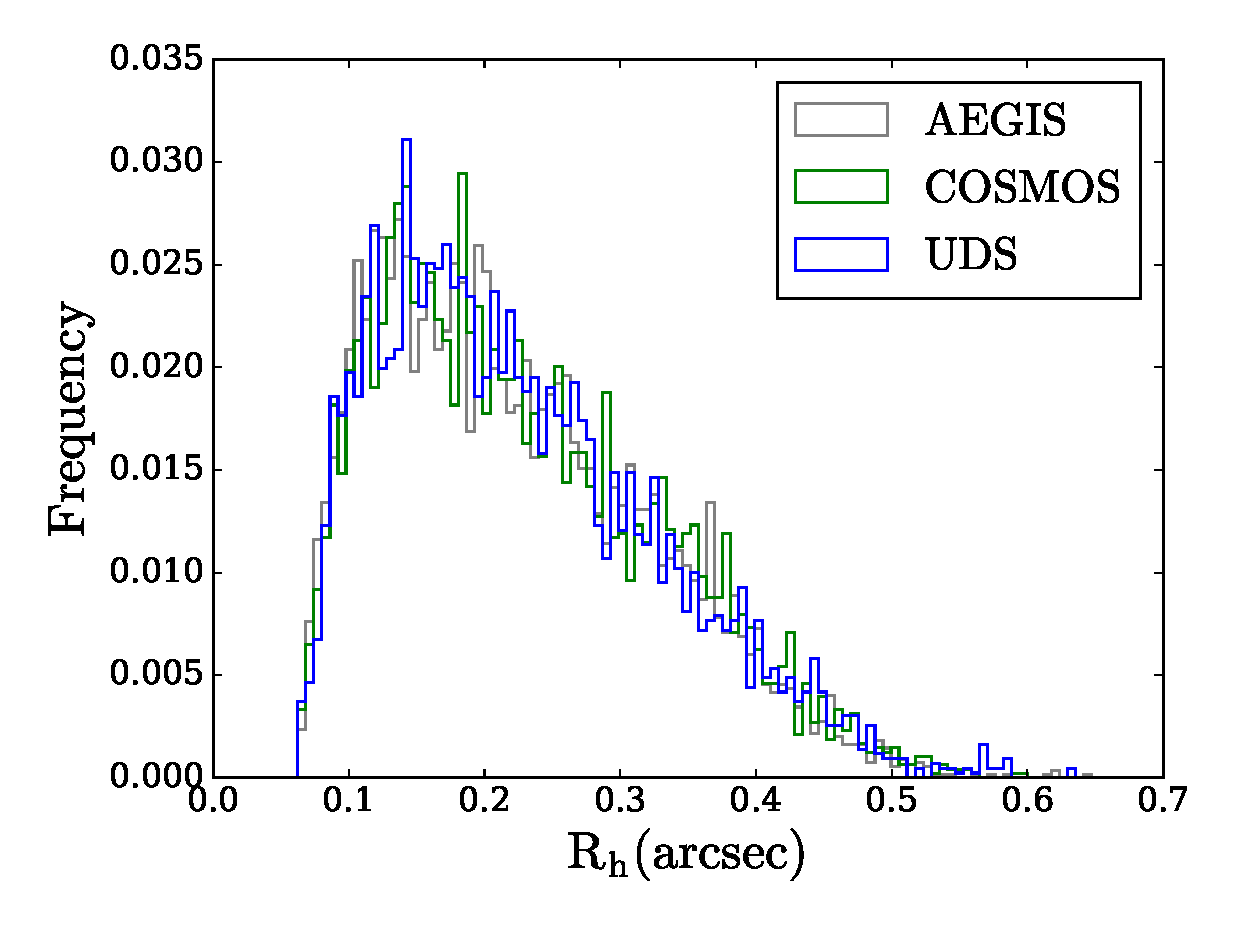
\includegraphics[width=5.0cm]{zhisrh.eps}
    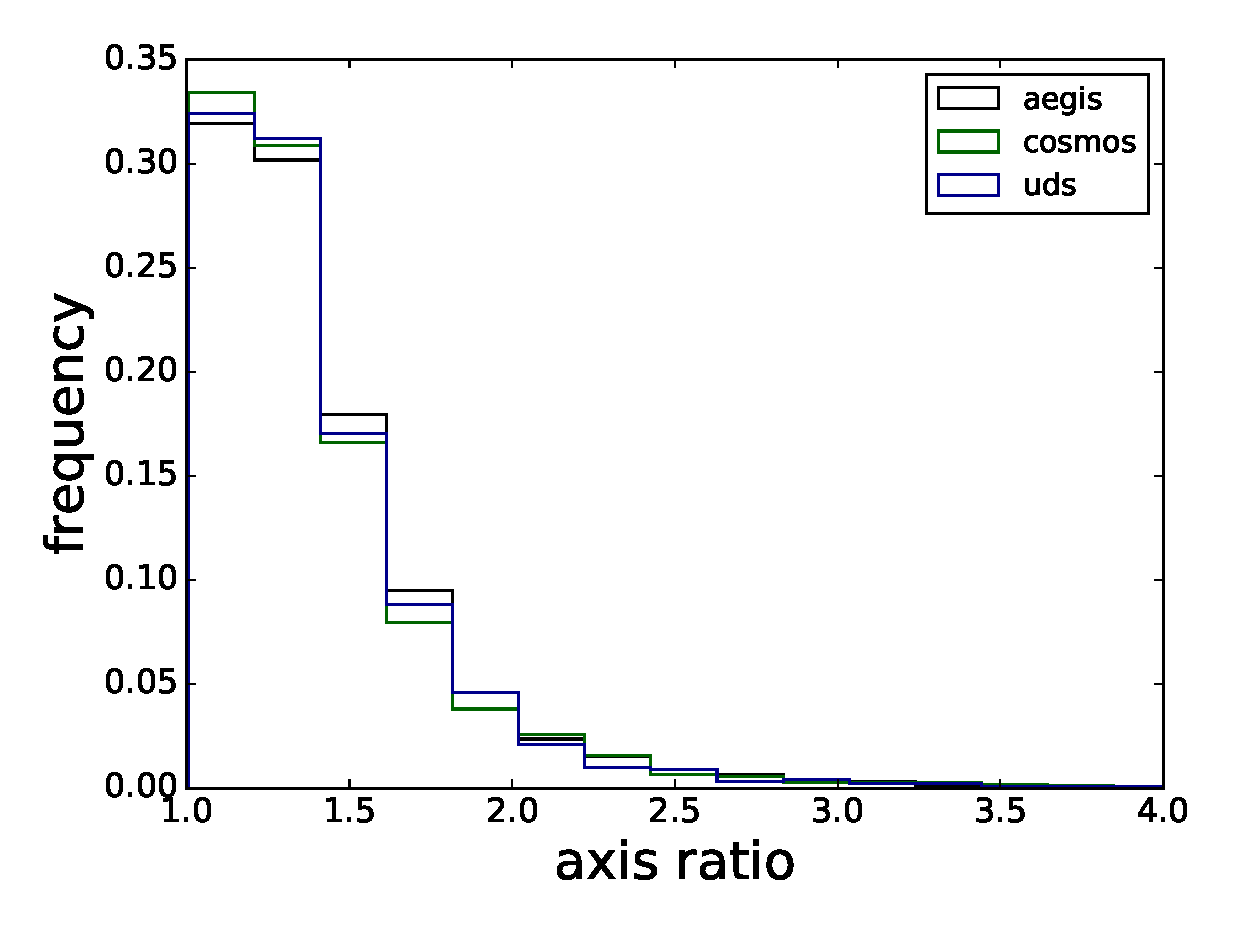
\includegraphics[width=5.0cm]{zhisratio.eps}
    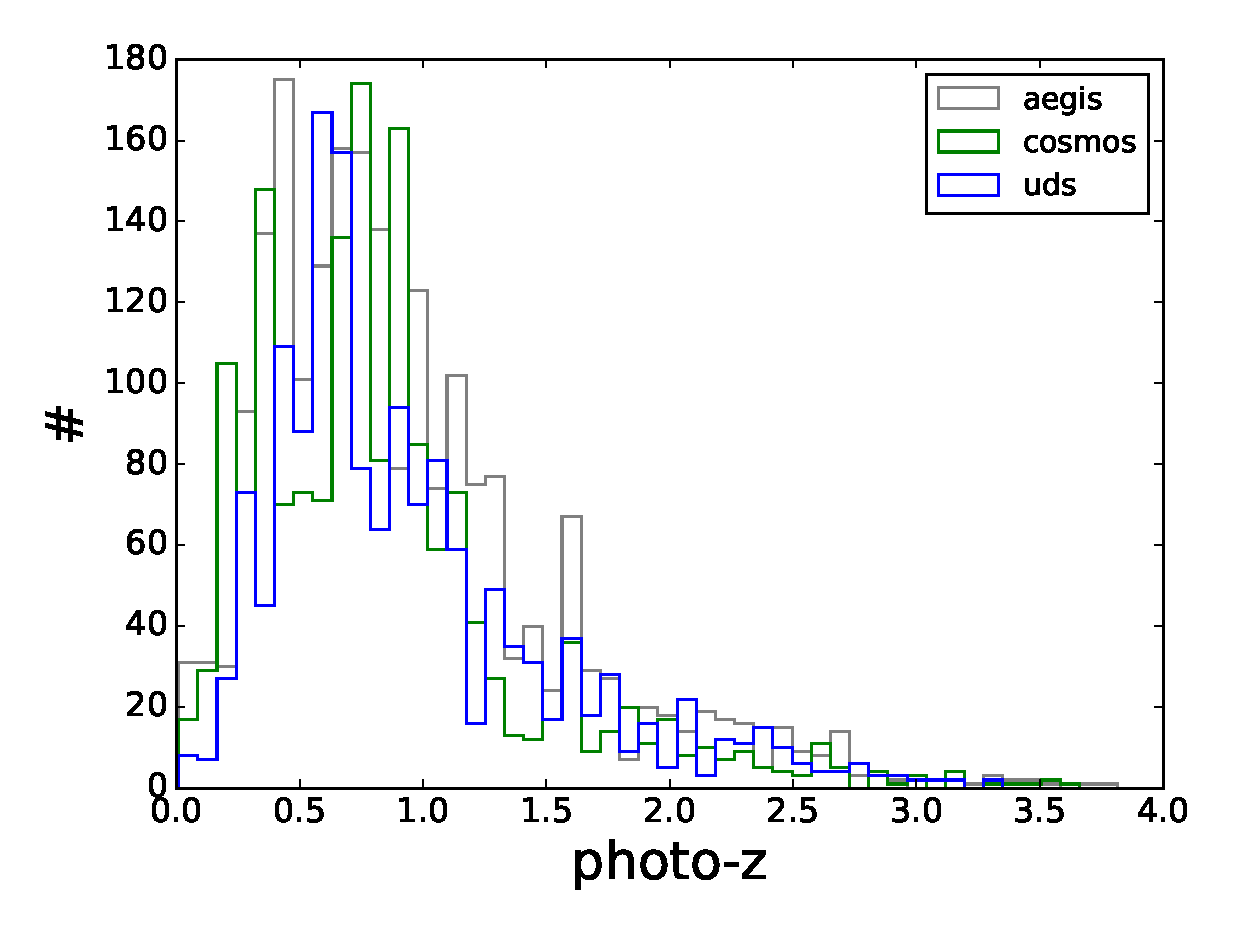
\includegraphics[width=5.0cm]{zhisphotoz.eps}
    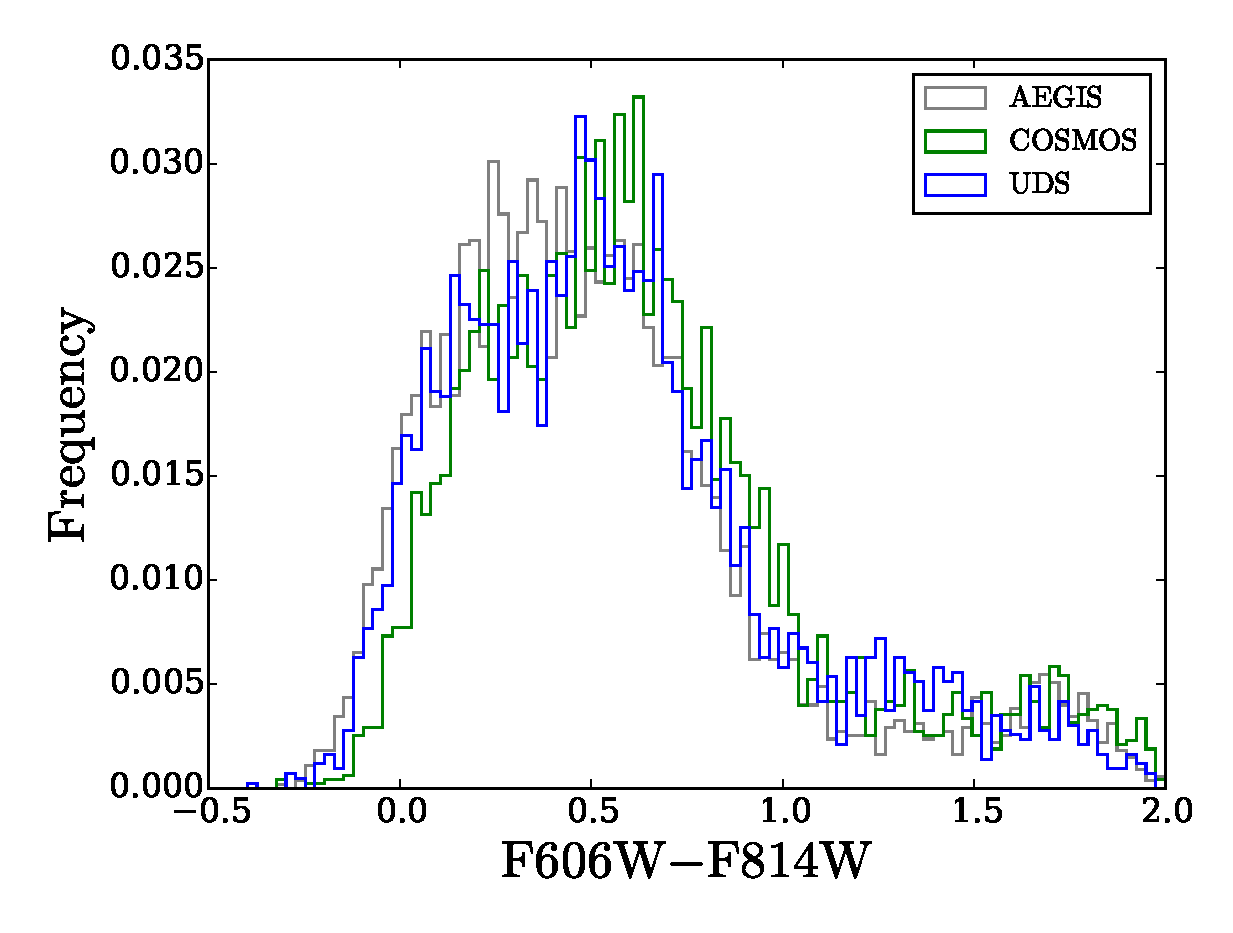
\includegraphics[width=5.0cm]{zhiscolor.eps}}
  \caption{The histogram for basic galaxy properties in our
    sample. The lines with different colours represent galaxies from
    different catalogues (AEGIS, COSMOS, UDS). From left to right: half
    light radius, axis ratio, photometric redshift, and colour
    ($m_{V-I}$).}
  \label{fig:datapro1}
\end{figure*}
%

\subsection{CG bias from CANDELS}
We estimate the CG bias following the same procedure for the simulated galaxy:
\begin{itemize}
  \item
    fit the galaxy using one Sersic component for both band
    images. Some constraints such as Sersic index ($0.5<n<3.5$),
    effective radius ($1<r_e<50$ pixel) and axis ratio ($0.6<q<1.0$)
    are adopted in Galfit.
  \item
    interpolate the SED on each pixel of the galaxy image, and
    generate the galaxy at each wavelength (Eq.\ref{eq:linearitp} -
    \ref{eq:lineareq}), and then integrate over the wavelength to
    simulate the CG and NCG galaxy image.
  \item
    measure the shape of two images and calculate the bias $m$. We
    also apply $6$ different orientation of the images in order
    to reduce the intrinsic shape noise.
\end{itemize}
%
In Fig.\ref{fig:cgbhis}, we show the histogram of the CG bias. The CG
bias in most of the galaxies is smaller than $0.01$ ($94\%$).  We did
not perform averaging as we did for the simulated noisy images, which
can further reduce the scatter of the bias. Thus the actual bias,
especially the scatter in the sample, is smaller. In the bottom
panel, we estimate the CG bias using a larger weight function
($2r_h$). As one expected, the bias decreases by about one order of
magnitude.

Three PSF models from TinyTim, which are the same as in the previous
section, are used in the deconvolution of CANDELS data. There is small
difference among the three since the three PSF models have similar
size. The following results are shown using the first PSF model from
TinyTim. 
%
%The red line show the CG bias if we perform lensing instead of shearing
%the images. We can see that the bias becomes larger, and the effect is
%stronger than the PSF variations. However, it is highly possible that we
%overestimate the flexion and the effect due to that, since we did not
%consider the real lens property. In the rest, we only show the result using
%shearing.

%
\begin{figure}
  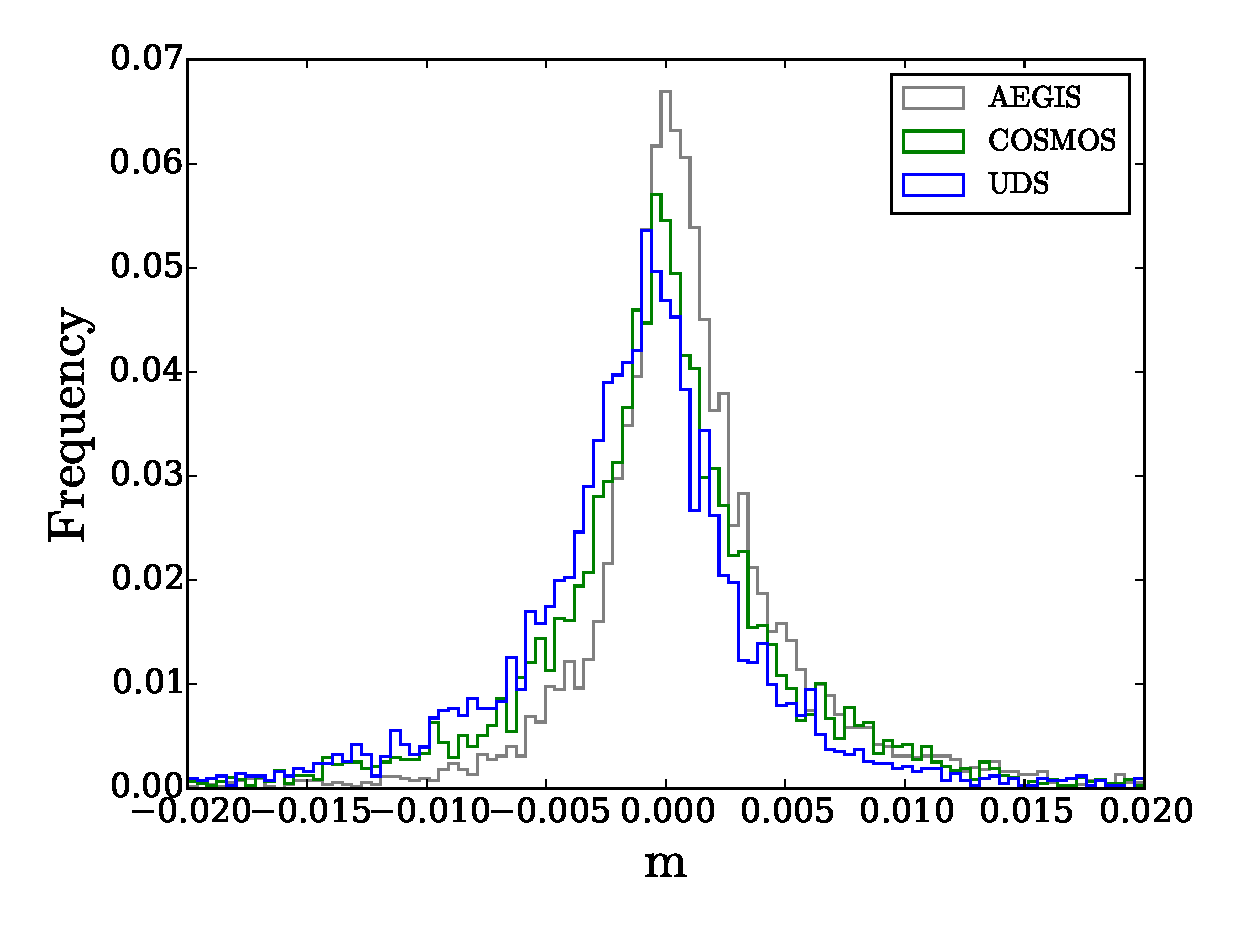
\includegraphics[width=7.0cm]{zhiscgb.eps}
  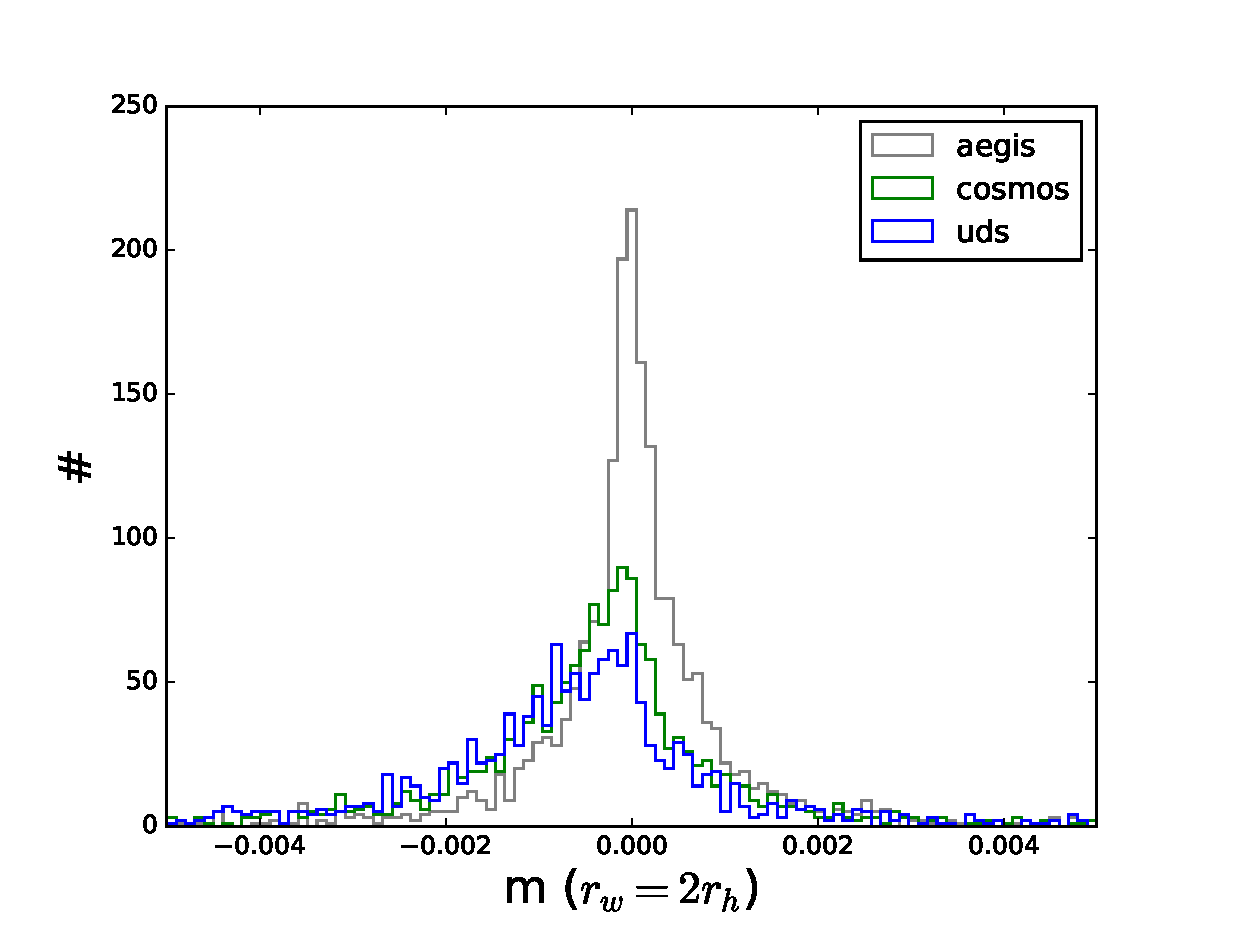
\includegraphics[width=7.0cm]{zhiscgbno.eps}
\caption{CG bias histogram from CANDELS: different colours show the
  result from three catalogures. In the bottom panel we show the CG
  bias using different weight function ($r_w = 2r_h$).  }
\label{fig:cgbhis}
\end{figure}
%
%\begin{figure}
%  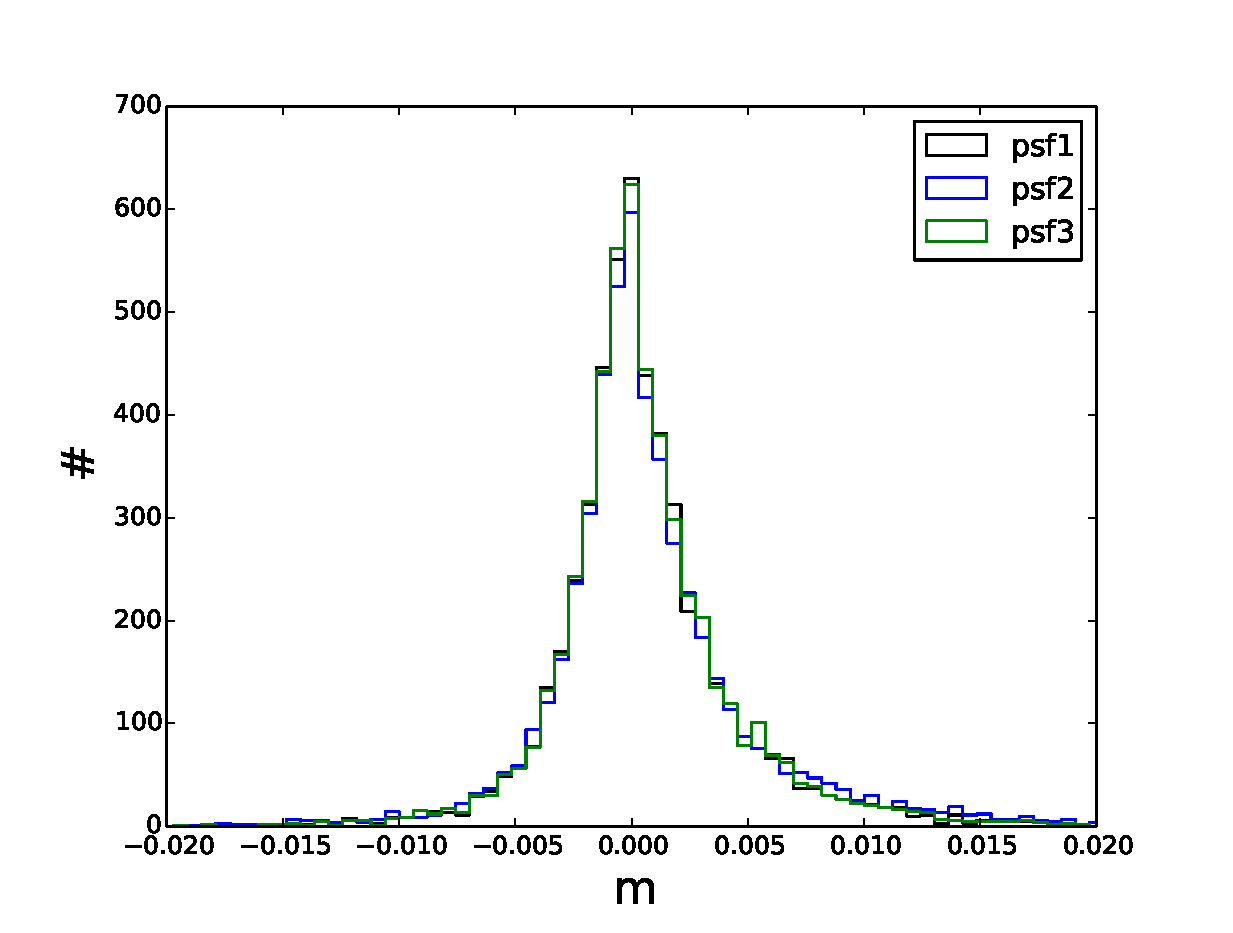
\includegraphics[width=7.0cm]{zcgbhis_psf.eps}
%  \caption{CG bias histogram of CANDELS using three different PSF
%    models from TinyTim.}
%  \label{fig:candelspsf}
%\end{figure}
%
\begin{figure}
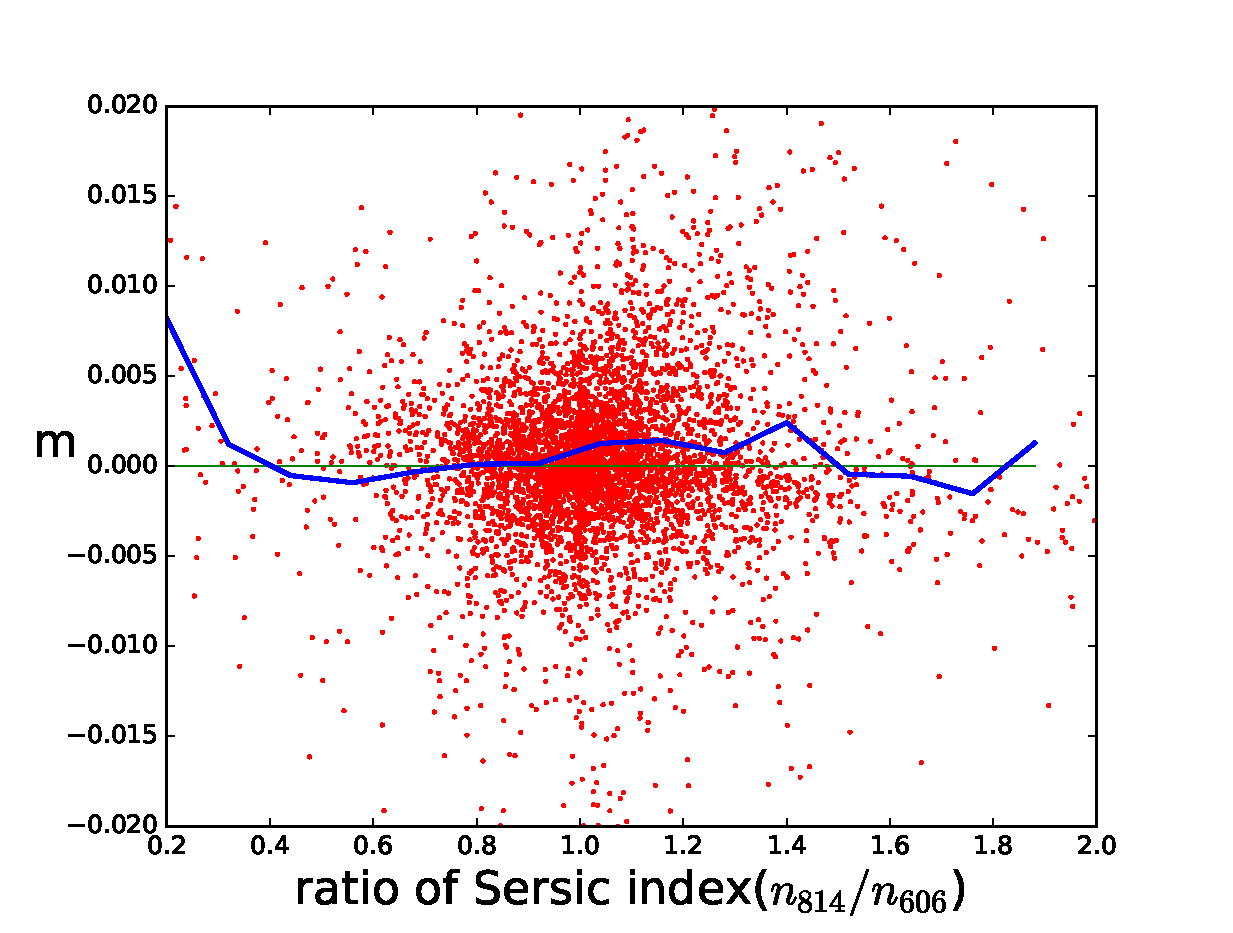
\includegraphics[width=7.0cm]{zcgb-ne17.eps}
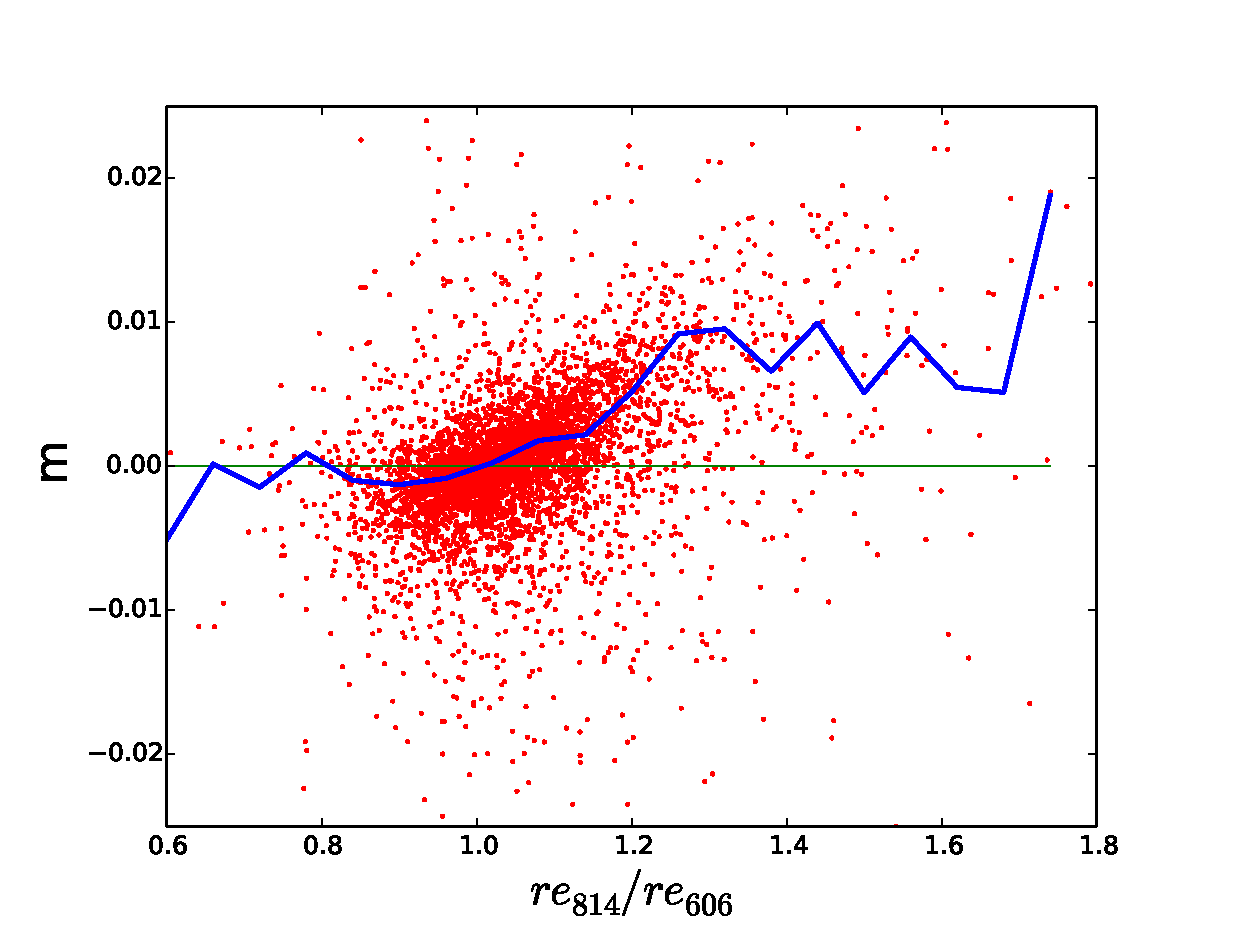
\includegraphics[width=7.0cm]{zcgb-re17.eps}
\caption{CG bias as a function of galaxy properties: ratio of Sersic
  index between two band (top) and effective radius between two bands
  (bottom). The blue lines are the average CG bias over the parameter
  bins.}
\label{fig:cg2fitpar}
\end{figure}
%
\begin{figure}
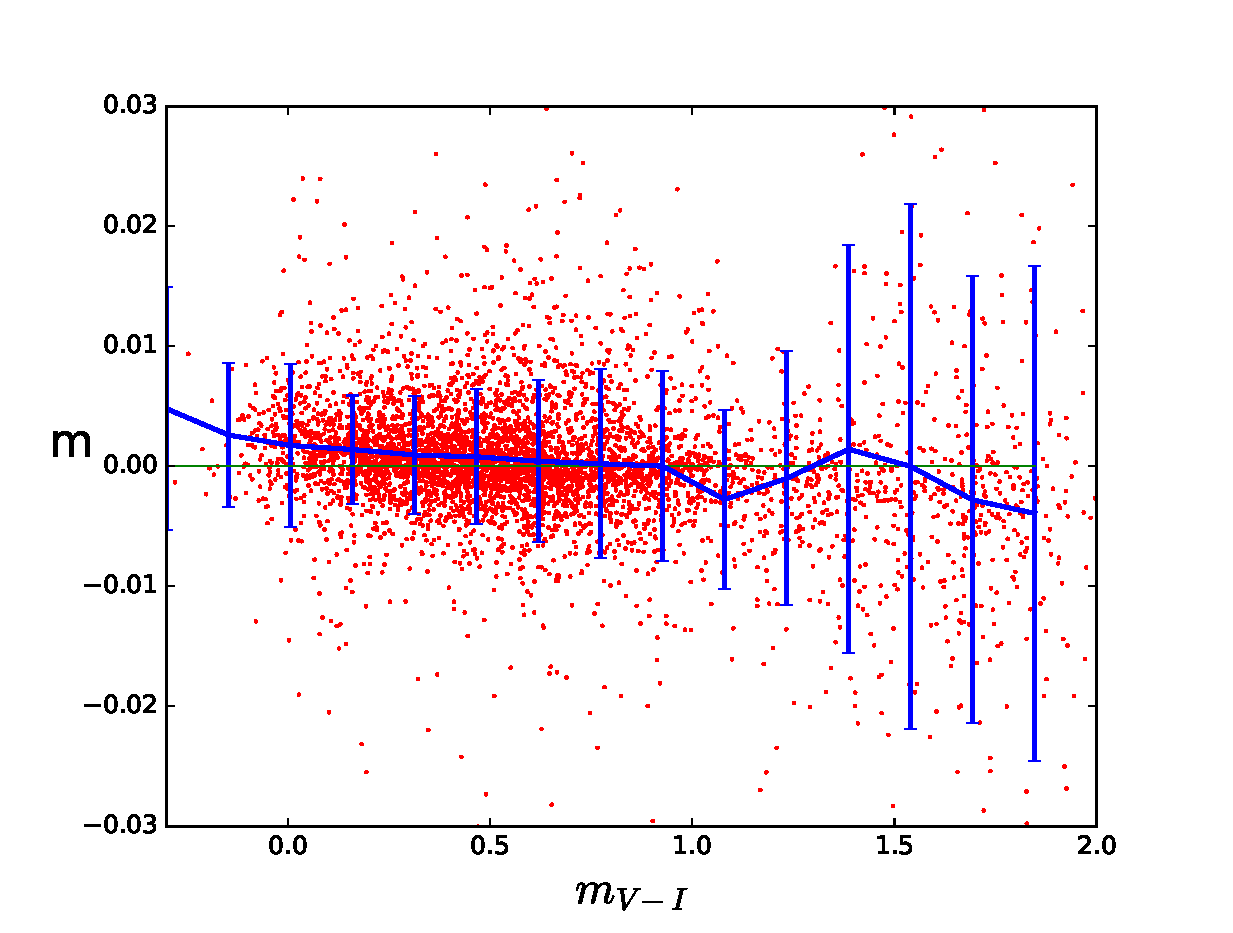
\includegraphics[width=7.0cm]{zcolor17.eps}
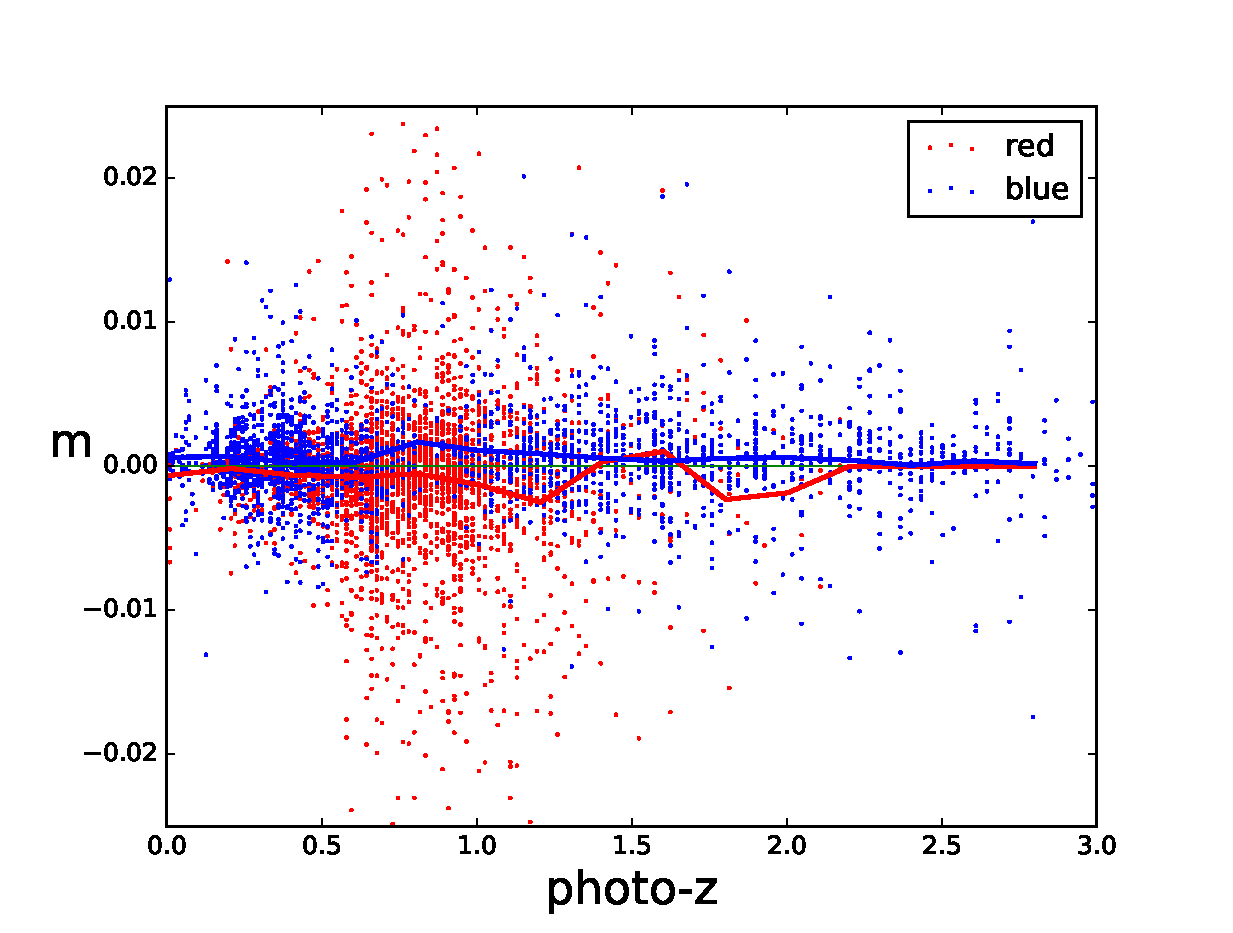
\includegraphics[width=7.0cm]{zphotoz17.eps}
\caption{CG bias as a function of galaxy properties, top: color
  ($m_{V-I}$), bottom: photo-z. In the bottom panel, the red and blue
  points are the bias for red ($m_{V-I}>0.5$) and blue ($m_{V-I}<0.5$)
  galaxies respectively. The lines are the average CG bias in the
  redshift bins.}
\label{fig:cg2color}
\end{figure}
%
\begin{figure}
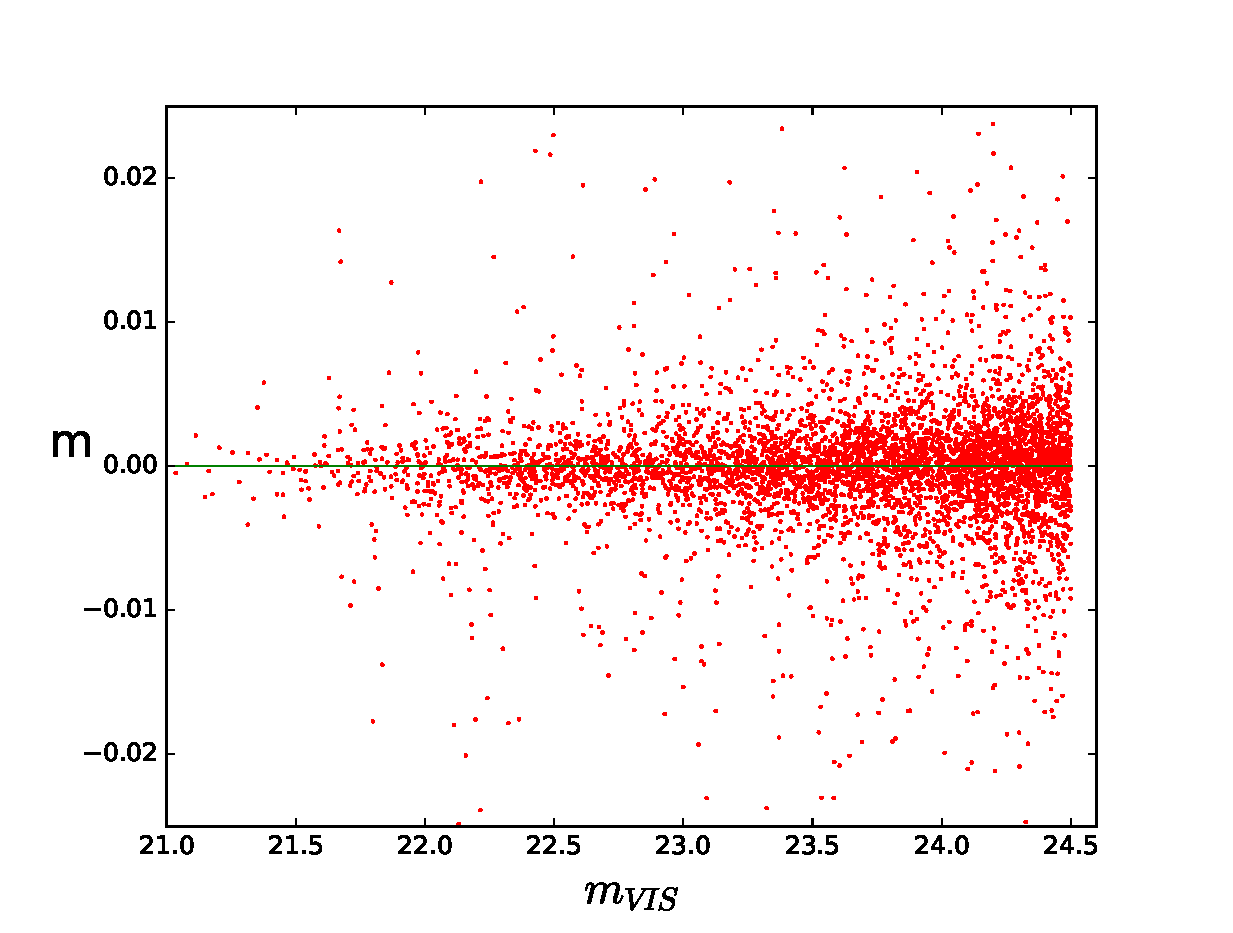
\includegraphics[width=7.0cm]{zcgb-magt17.eps}
\caption{CG bias as a function of mock VIS magnitude. }
\label{fig:cg2magvis}
\end{figure}
%
\begin{figure}
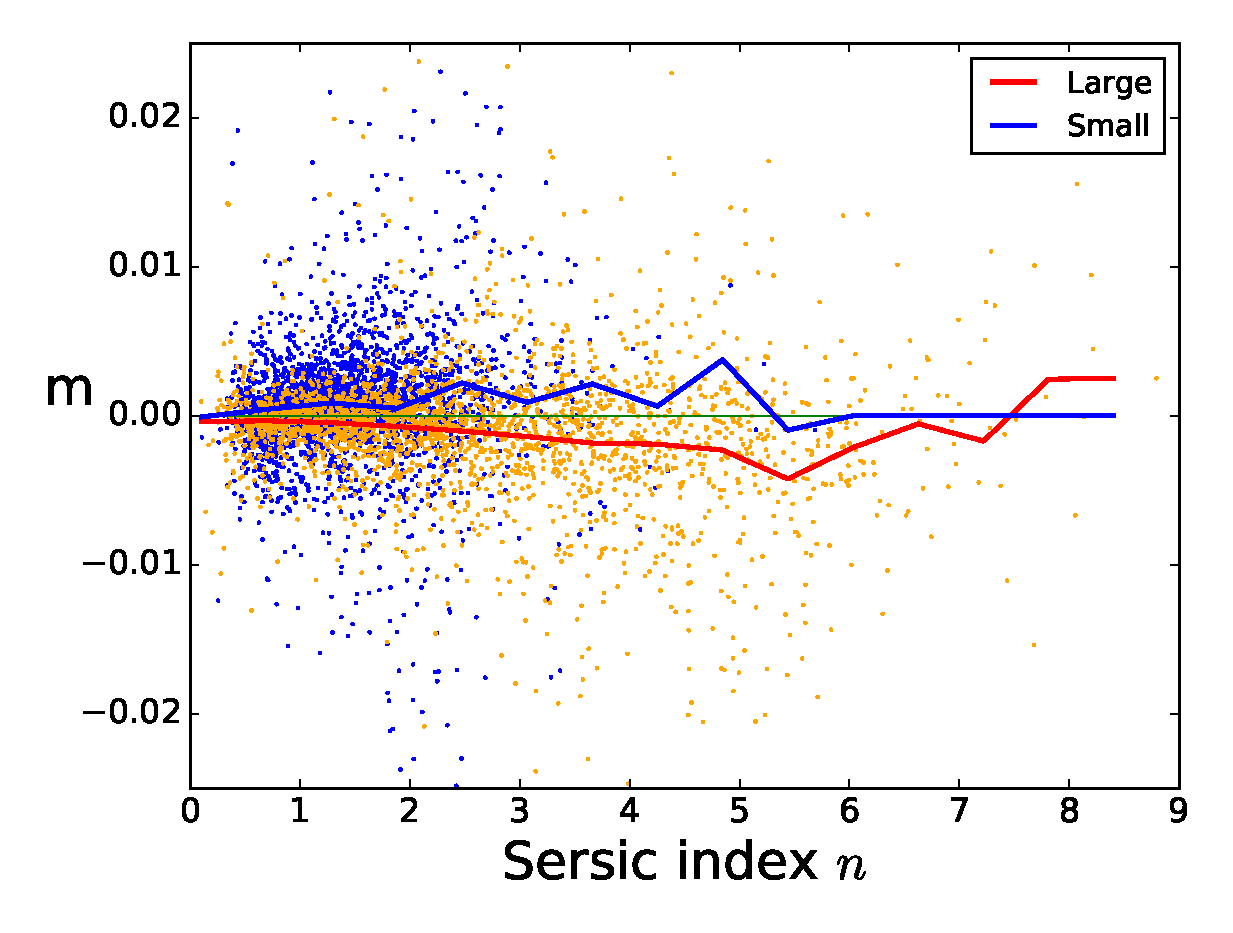
\includegraphics[width=7.0cm]{z2s-ne17.eps}
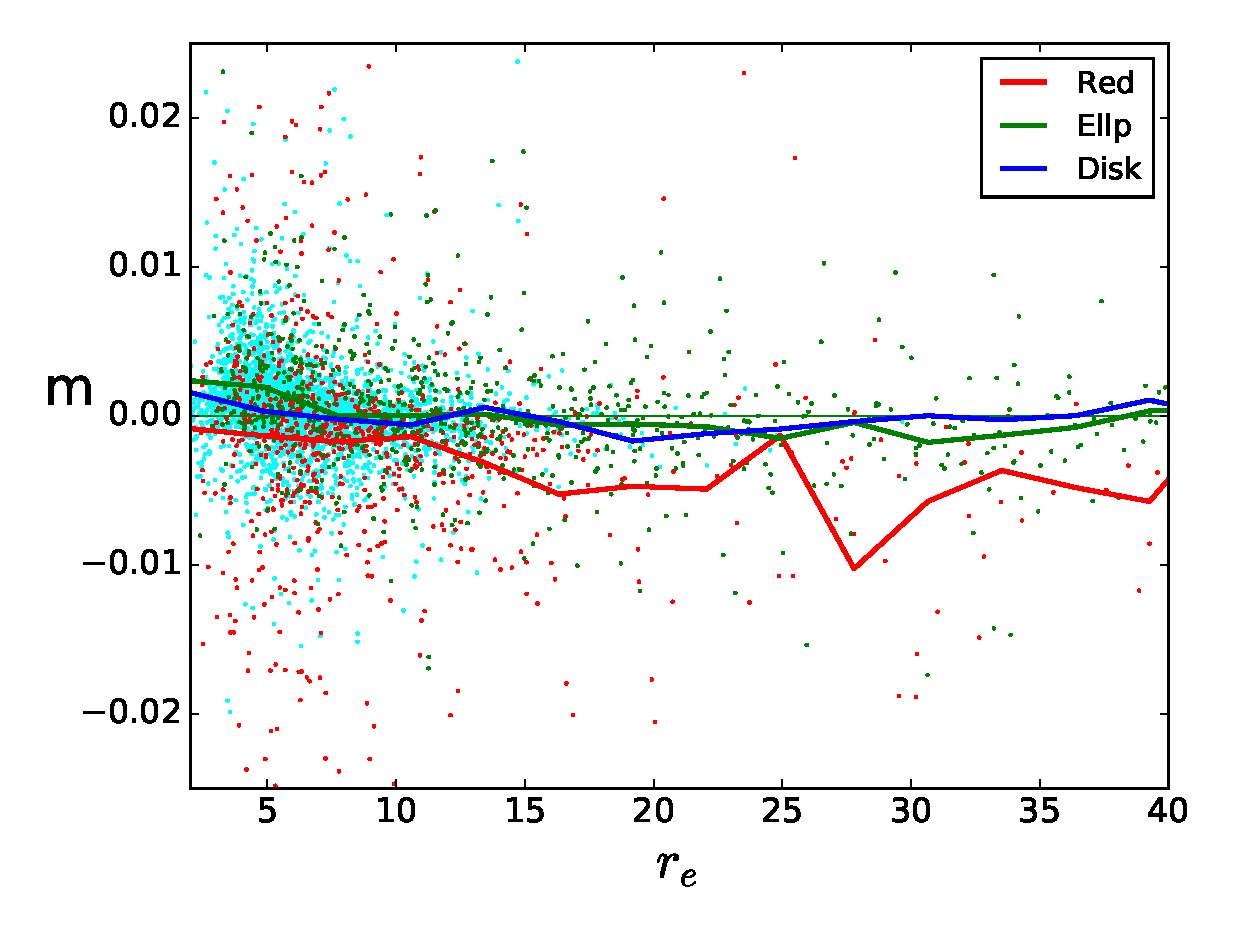
\includegraphics[width=7.0cm]{z2nscl-re17.eps}
\caption{CG bias with Sersic index (top) and effective radius (bottom)
  from the mock VIS images. The unit of radius is a pixel ($=0.05$
  arcsec). In the top panel, the blue (red) is the average of small
  (big) galaxies. In the bottom panel, the red line is average bias of
  red galaxy ($m_{V-I}>1$); the green line is that of elliptical
  galaxy ($n_{Sersic}>2.75$); the blue line is for the disk galaxy.}
\label{fig:cg2re}
\end{figure}
%
In order to find a quick estimation for the CG bias, we try to find
the relation between CG bias with galaxy parameters. In
Fig.\ref{fig:cg2fitpar}, one can see the CG bias with the fitting
parameters from two band images. On one side, we
do not find any obvious relation between CG bias and ratio of Sersic
index from two bands. On the other side, we see that
there is an approximately linear relation between the ratio of
effective radii and CG bias.  Moreover, one expect that when
$r_{e606}=r_{e814}$ and $n_{606}=n_{814}$, the CG bias in principle
will be vanish, since the identical images from two bands will not
have a colour gradient. In Fig.\ref{fig:cg2fitpar}, the blue lines are
the binned average CG bias. In the bottom panel, one can see that the
average bias meets zero at $r_{e814}/r_{e606}=1$, as
expected. However, in the Euclid VIS image survey, we will have only
one band images, we thus need other methods for the bias estimation.


In Fig.\ref{fig:cgbhis}, the galaxies in AEGIS field have more
positive CG bias than the galaxies in the other two. The colour
distribution in AEGIS is different from the other two as well, which
suggests the correlation between the CG bias and the colour of the
galaxy. In Fig.\ref{fig:cg2color}, we show the relation between the CG
bias and the colour of the galaxies (here the colour is the magnitude
different between $V$ and $I$ band). The bias is inversely
proportional to the colour of the galaxies. The galaxy sample is split
into two groups according to their colour: the red galaxies
($m_{V-I}>0.5$) and the blue ones ($m_{V-I}<0.5$). They are shown in
the bottom panel of Fig.\ref{fig:cg2color} as a function of
redshift. Most of the red galaxies are located at moderate redshifts,
mainly between redshift $[0.5,1.0]$, while the blue galaxies are
either at the lower redshift ($z<0.5$) or higher redshift
($z>1.0$). The CG bias in red galaxies are obviously more negative
than that of the blue ones. The number density of very red galaxy 
($m_{V-I}>1$) is low and the scatters of the bias are large.

In Fig.\ref{fig:cg2magvis}, we show the bias as a function of our mock VIS
magnitude ($m_{VIS}$). There is no obvious dependence on $m_{VIS}$. Although
the actual $m_{VIS}$ is different from our linear approximation, also
the filter transmission are different of two telescope, the correlation
between $m_{VIS}$ and CG bias will not be an accuracy method for CG bias.


Moreover, we stack the images from two bands as our mock VIS band
images.  Fig.\ref{fig:cg2re} shows the CG bias with the Sersic index
and the effective radius fitted from the VIS images. In the top panel,
we divide the sample into two groups by the fitted effective radius,
either larger or smaller than $0.35$ arcsec. The small (large)
galaxies are shown by the blue (orange) points, and the blue (red)
line is the bin average.  The large galaxies cover a large range of
Sersic index, have negative average CG bias. Most of small galaxies
have small Sersic index ($<2.5$). The bias of small galaxies are
positive and approximately proportional to the Sersic index. The
scatters of the bias for both large and small galaxies increase with
the Sersic index.
%
In the bottom panel, the galaxies are divide into three groups: the
first is red galaxy whose color is large ($m_{V-I}>1.0$); the second
and third group are the rest galaxies either with large Sersic index
($n>2.25$, elliptical galaxy) or small Sersic index (disk galaxy). The
solid lines show the bin average over effective radius. 
%
%\be
%\tilde{m} = a\,r_e+{b\over r_e}+c,
%\elabel{fitcgb}
%\ee
%
%where $r_e$ is the effective radius of the mock VIS image. For disk
%galaxy we have $a=3.8\times10^{-12}$, $b=0.022$, $c=-0.0066$, and for
%elliptical galaxy $a=0.00012$, $b=0.017$ and $c=-0.0069$. The disk
%galaxies have relatively smaller size and smaller CG bias, while the
%elliptical galaxies cover a large range of size and CG bias. Moreover,
%the elliptical galaxies have a stronger dependence on the effective
%radius.
%
We can see that the VIS image alone can also provide an rough
estimation for CG bias, but classification of the galaxies is
necessary. As shown in the figure, the disk galaxies have small bias,
small radius ($<1$ arcsec), and also small bias scatters. The
elliptical galaxies cover large radius range, and the bias is larger
than the disk ones. The bias in red galaxies are significant, and
mainly negative. The scatters of red galaxies are larger than the
other two kinds of galaxies.
%
The multi-band photometry can definitely provide information on the CG
bias, since the colour and colour gradient are correlated
intrinsically during the evolution of galaxy. Moreover, the multi-band
information is required for the photometric redshift study. One can
obtain that for free to calibrate the CG bias. Although the dependence
on the multi-band is different between photometric redshift and CG
bias, the experience from photometric redshift can be used for CG
bias, such as some machine learning algorithms.


We calculate the average bias and the dispersions over the redshift
bins for both red ($m_{V-I}>0.5$) and blue galaxies
(Table\,\ref{table:calibration}). The red galaxies are mainly located
between redshift $(0.4,1.2)$, while the blue galaxies are low density
in redshift $(0.8,1.2)$. The bias from red galaxies are significantly
smaller than that of blue galaxies, as one expected, the colour
gradient in the elliptical galaxies are smaller. The dispersions of
the bias in each bin are large, which probably indicate that in each
bin there are several kinds and sizes of galaxies.  Therefore, in
order to calibrate the bias with high precision, one need bigger
galaxy samples. From our simulation, we need about $200$ galaxies for
one type of galaxy in every redshift bin. If we make rough bins, for
instance, 2 types of colour: red and blue; 5 different sizes from
about $0.1$ arcsec to $1.0$ arcsec (Fig.\ref{fig:cg2re}), and 5
redshift bins, at least $10 000$ galaxies are required.  For more
realistic SED classifications and redshift bins, several times larger
sample are also necessary.


\begin{center}
\begin{table}
  \begin{tabular}{llll}
    \hline
    photo-z    &$Number$  &$\bar{m}$  &$\sigma_m$ \\
    \hline
    $0-0.4$   &187  &$-1.3\times10^{-3}$  &$0.012$\\
    $0.4-0.8$  &1415 &$-7.6\times10^{-4}$  &$0.011$\\
    $0.8-1.2$  &1116 &$-1.0\times10^{-3}$  &0.017\\
    $>1.2$  &245  &$-2.1\times10^{-3}$  &0.015\\
    \\
    $0-0.4$  &667  &$6.6\times10^{-4}$  &0.0026\\
    $0.4-0.8$ &513  &$2.8\times10^{-4}$  &0.0028\\
    $0.8-1.2$ &187  &$1.2\times10^{-3}$  &0.0041\\
    $>1.2$  &935  &$5.4\times10^{-4}$  &0.0046\\
    \hline
  \end{tabular}
  \caption{\label{table:calibration}The number, average CG bias and dispersion in redshift bins for blue (bottom half) and red (top half) galaxies. }
\end{table}
\end{center}

%\be
%c=m{e_{\rm PSF} \over P_{\gamma}P_{ePSF}},
%\ee
%follow Massey $P_{ePSF}=1$, $P_{\gamma}=0.93$ and using a conservative choice, which corresponds to the maximum value for the polarization allowed for the Euclid PSF $e_{PSF}=0.07$.


\section{Summary and Discussion}
In the image survey for weak gravitational lensing, the wide band
filter can provide high signal-to-noise images and large coverage of
redshift range. There is however a shape bias due to the chromatic
shape of galaxy and the PSF, which is named as colour gradient
bias. For very wide band surveys, such as Euclid, this effect can
cause a non-negligible bias.
%
In this work, we exam such a kind of bias in measuring the shape of
a galaxy using both simulated images and real data taken from the HST ACS
CANDELS survey.  In the simulated galaxy images, we confirm the bias
behaviour from previous results (ES13). We further apply the calibration
method to the noisy images in the simulations, and find that with
reasonable signal-to-noise ratio (SNR$=15$) and numbers of galaxies ($300$
images for one type of galaxy in one redshift bin), we can estimate
the CG bias to a high precision. However, the underestimate cannot
be avoided due to strong emission lines, or the uneven SED of source
galaxies. Moreover, the SNR of the simulated images in two
bands are assumed to be the same. In reality, the signal-to-noise in
different bands are correlated to the SED of the galaxies.

We also apply the calibration method to the galaxy images taken by HST
in two filters (F606W, F814W). In the estimation using CANDELS data,
we find that most of the CG bias ($|m|$) is smaller than $0.01$.  As
we find from simulated images, the estimation using noisy image has a
large scatter, thus the CG bias in reality may be smaller than that
shown here.
%
In our sample of galaxies, the CG bias shows a correlation with the
colour of galaxies, and a linear relation with the ratio of two band
images.  In case there is only one wide band image, one can also
classify the galaxy by their Sersic index. The galaxies with small
Sersic index, i.e. disk-like, have smaller CG bias. On the other hand,
those with large Sersic index have large bias and also bias variation.
Since the bias depends on the size of the galaxies as well, we can
have an approximate fitting formula for the bias for different galaxy
morphology. The fitting is limited to the galaxies in our sample,
further investigation for different type of galaxies is necessary. The
photometry from several bands, which will be used to estimate the
redshift, can be also use for the CG bias analysis. Although the
redshift dependence is not significant in our sample of galaxies, this
may not be the case for a larger survey. In order to fully calibrate
the bias for different redshift, a larger sample is essentially
necessary. Moreover, in the weak lensing study, the colour of galaxies
can be also used for the intrinsic alignment analysis. There is a
potential correlation between the CG bias and the intrinsic alignment
noise.
%It maybe interesting to explore more about galaxy morphology.
%Moreover, only two galaxy models are used in the simulation for the
%source galaxy images.

It has been shown that colour gradients depend on the environment
where galaxies reside, with steeper colour gradients in poor rather
than rich clusters \citep[e.g.][]{2005ApJ...626L..19L}, which is
possible due to the different processes during galaxy formation. Close
galaxy pairs or nearby bright star(s) will also cause
brightness/colour gradient, which can affect our estimate for CG bias
as well. The significance of the environment to CG bias is not clear
and requires further study as well. Moreover, in the calibration we
linearly interpolate the SED on pixels from two bands. Some advanced
method to estimate the SED \citep[e.g.][]{2016A&A...589A...2J} may
help to improve the calibration of the bias.

In this work, we use the brightness moments to estimate the
ellipticity of the galaxy. The PSF correction is not taken into
account. The bias thus will appear in any method of measurement.
However, the bias using the measurement method for real data
will be different, since every method has its own property and weight
function. The CG bias will have method-dependent properties as well,
although they will in principle have same dependence on the colour
gradient of the galaxy images. As the first step of the CG bias
analysis, we did not adopt any specific method in order to obtain
general properties of the CG bias. Before the real analysis of Euclid
data, one needs to study the bias with specific methods and simulated
images with real properties in the Euclid weak lensing survey.

%
%Moreover, as we point out that higher order image distortions, such as
%flexion may increase the CG bias. It can be seen from our analysis
%using both simulated and CANDELS data. Although the higher order
%effect can be neglected most times, it can still significantly
%increase the CG bias when the source images are located close to the
%strong lensing region. Therefore, such a kind of effect may cause
%significant bias in the strong lensing analysis using wide band
%images. In galaxy-galaxy lensing and cluster lensing, one needs to
%be careful about such higher order effects as well.

\section*{Acknowledgments}

We would like to thank Emiliano Merlin, Marco Castellano for helping on SExctractor and Galfit, Gary Berstein, Adam Rogers, Junqiang Ge and also in general, the members of the Euclid Consortium for useful discussions.
XE and VFC are funded by Italian Space Agency (ASI) through contract Euclid -IC (I/031/10/0) and acknowledge financial contribution from the agreement ASI/INAF/I/023/12/0. XE is also partly support by NSFC Grant No. 11473032. JR is supported by JPL, which is run by Caltech under a contract for NASA, and is supported by grant NASA ROSES 12-EUCLID12- 0004. The fast Fourier transforms are supplied by the FFTW library \citep{fftw05}. We use CFITSIO \citep{1999ASPC..172..487P} for the FITS file.
%This study makes use of data from AEGIS, a multiwavelength sky survey conducted with the Chandra, GALEX, %Hubble, Keck, CFHT, MMT, Subaru, Palomar, Spitzer, VLA, and other telescopes and supported in part by the %NSF, NASA, and the STFC.

\appendix
\section{Ratio of Moment vs. PSF convolution}
In general, the PSF correction will cause extra bias in the shear
estimation.  In order to isolate the CG bias, we measure the
brightness moments without applying any PSF correction methods in this
work, i.e. the CG bias will appear in any method.  Moreover, the
definition of our CG bias uses the ratio of ellipticity from images,
thus the estimate for the CG bias will not be changed by the
convolution of a small PSF.  Let us denote the quantity with prime for
those convolved with PSF, i.e.,
%
\be
I'(\theta) = \int \d^2 \psi I(\theta) P(\theta-\psi).
\ee
%
The weighted brightness moment can be written as
%
\bea
Q_{ij} &=& \int \d^2 \theta W(\theta)\, f_{ij}(\theta) I(\theta ),\\
Q_{ij}' &=& \int \d^2 \theta W(\theta)\, f_{ij}(\theta)\int \d^2\psi I(\psi) P(\theta-\psi),
\eea
%
where $f_{ij}(\theta)$ is the function to characterize the brightness
moments, e.g. $f_{ij}(\theta)=\theta_i\theta_j$ for the second order
moment. We can replace the variable $\psi$ by $r=\theta-\psi$, and
Taylor expand with respect to $\psi$. Then the moment becomes
%
\bea
Q_{ij}' &=& \int \d^2 \theta W(\theta)\, f_{ij}(\theta) \int \d^2r I(\theta-r) P(r)\\
&\approx &\int \d^2 \theta W(\theta) f_{ij}(\theta) \int \d^2r P(r) \eck{I(\theta)-{\partial I(\theta) \over \partial r}r}, \nonumber \\
&=&Q_{ij} \int \d^2r\,P(r) - \int \d^2\theta\, W(\theta) f_{ij} \int \d^2r\, P(r) {\partial I\over \partial r}r.\nonumber
\eea
%
The integral of $P(r)$ in the first term independent of the image of
the galaxy, and equals to unity for normalised PSF. In case of
circular symmetric PSF or the asymmetry is small, the second term can
be neglect. $Q_{ij}'\approx p Q_{ij}$, where $p$ is only determined
by the size of PSF. Thus, for small PSF we have the approximation
%
\be
{Q^{cg'}_{ij} \over Q^{ncg'}_{ij}} \approx
{Q^{cg}_{ij} \over Q^{ncg}_{ij}}, \;
\ee
%
which means that the small circular PSF will not change the CG bias in
our definition.
%In Fig.\,\ref{fig:psftest}, we compare the CG bias before and after the deconvolution
%with the effective PSF. One can see that the two lines are almost overlapped.
%
%\begin{figure}
%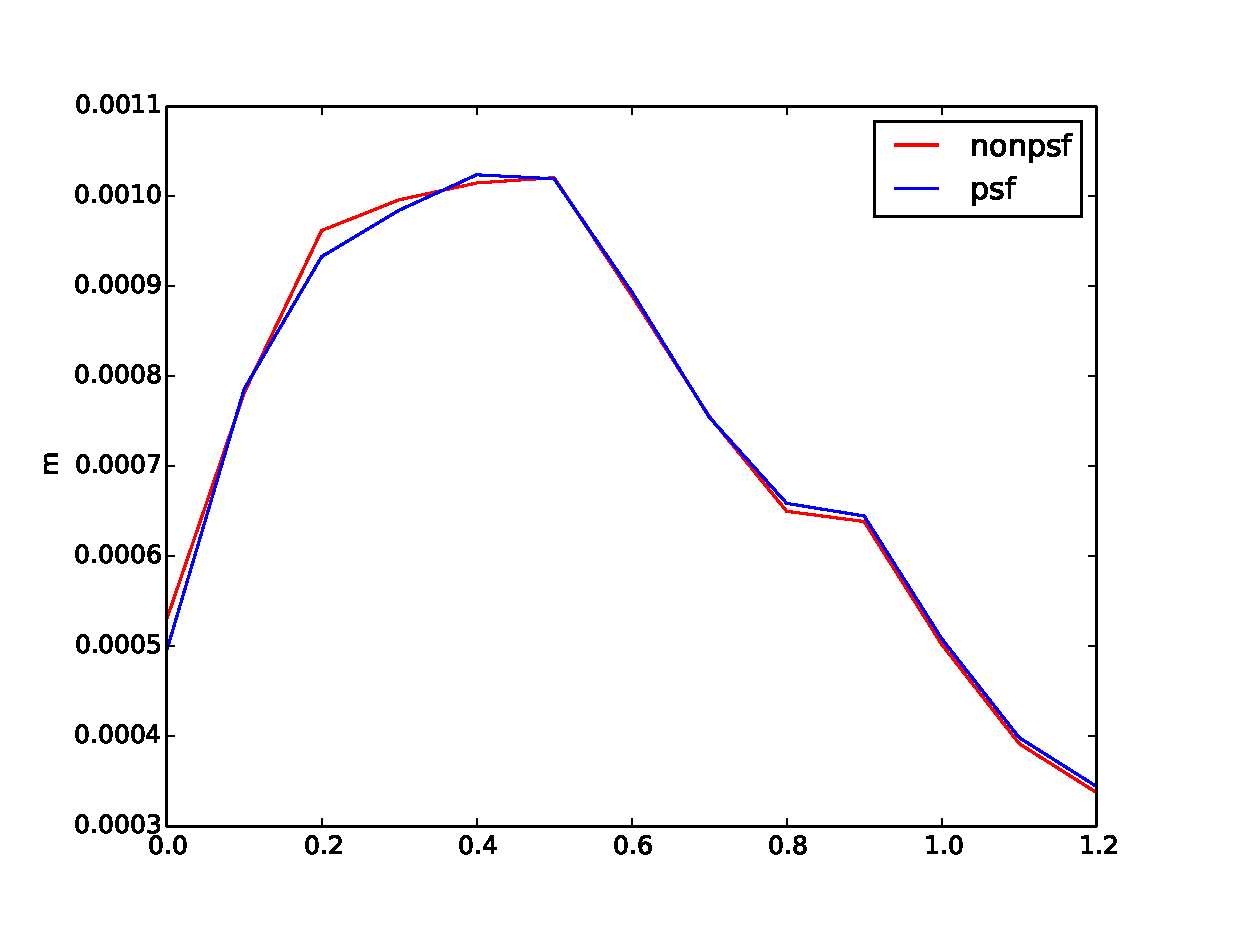
\includegraphics[width=7.0cm]{zpsft1.eps}
%\caption{CG bias before (blue) after (red) deconvolution of the integrated PSF.
%}
%\label{fig:psftest}
%\end{figure}
%

\bibliographystyle{aa}
\bibliography{../bib/refbooks,../bib/lens,../bib/flexion,../bib/shear,../bib/stronglens,../bib/galaxy,../bib/survey,../bib/stats}

\end{document}
